\documentclass[review]{elsarticle}

\usepackage{lineno,hyperref}
\modulolinenumbers[5]

\usepackage{amsmath}
\usepackage{amsfonts}
\usepackage{multirow}
\usepackage{subcaption}

\PassOptionsToPackage{dvipsnames}{xcolor}
\usepackage{tikz}
\usetikzlibrary{arrows,positioning,fit,petri,backgrounds,decorations.pathmorphing}
\usepackage{pgfplots}
\usepgfplotslibrary{statistics}

\usepackage{picins}
\usepackage[dvipsnames]{xcolor}

\journal{Computer Speech \& Language}

%%%%%%%%%%%%%%%%%%%%%%%
%% Elsevier bibliography styles
%%%%%%%%%%%%%%%%%%%%%%%
%% To change the style, put a % in front of the second line of the current style and
%% remove the % from the second line of the style you would like to use.
%%%%%%%%%%%%%%%%%%%%%%%

%% Numbered
%\bibliographystyle{model1-num-names}

%% Numbered without titles
%\bibliographystyle{model1a-num-names}

%% Harvard
%\bibliographystyle{model2-names.bst}\biboptions{authoryear}

%% Vancouver numbered
%\usepackage{numcompress}\bibliographystyle{model3-num-names}

%% Vancouver name/year
%\usepackage{numcompress}\bibliographystyle{model4-names}\biboptions{authoryear}

%% APA style
%\bibliographystyle{model5-names}\biboptions{authoryear}

%% AMA style
%\usepackage{numcompress}\bibliographystyle{model6-num-names}

%% `Elsevier LaTeX' style
\bibliographystyle{elsarticle-num}
\biboptions{sort&compress}
%%%%%%%%%%%%%%%%%%%%%%%


\def\x{{\mathbf x}}
\def\L{{\cal L}}

\definecolor{BoxCol}{RGB}{0,105,133}
\definecolor{BoxCol1}{RGB}{117,48,31}
\definecolor{BoxCol2}{RGB}{255,180,00}

\DeclareMathOperator*{\argmax}{arg\,max}
\newcommand{\symvec}[1]{{\mbox{\boldmath $#1$}}}
\newcommand{\symmat}[1]{{\mbox{\boldmath $#1$}}}
\newcommand{\mat}[1]{\mathbf{#1}}
\newcommand{\nat}{\mathbb{N}}
\newcommand{\real}{\mathbb{R}}
\newcommand{\setR}{\mathbb{R}}
\newcommand{\eg}{e.\,g.\xspace}
\newcommand{\ie}{i.\,e.\xspace}
\newcommand{\wrt}{w.\,r.\,t.\xspace}
\DeclareMathOperator*{\argmin}{arg\,min}
\newcommand{\bmu}{\mu \kern-0.65em \mu}

\newcommand{\ShiftedRight}[2]{\overset{#2 \rightarrow}{#1}}
\newcommand{\ShiftedLeft}[2]{\overset{\leftarrow #2}{#1}}
\newcommand{\FwdArrow}[1]{\overset{\rightarrow}{#1}}
\newcommand{\BwdArrow}[1]{\overset{\leftarrow}{#1}}
\newcommand{\secref}[1]{Section~\ref{#1}}
\newcommand{\figref}[1]{Fig.~\ref{#1}}
\newcommand{\tableref}[1]{Table~\ref{#1}}
\let\originaleqref=\eqref
\renewcommand{\eqref}{Eq.~\originaleqref}

\begin{document}


\begin{frontmatter}

%% Title, authors and addresses

%% use the tnoteref command within \title for footnotes;
%% use the tnotetext command for the associated footnote;
%% use the fnref command within \author or \address for footnotes;
%% use the fntext command for the associated footnote;
%% use the corref command within \author for corresponding author footnotes;
%% use the cortext command for the associated footnote;
%% use the ead command for the email address,
%% and the form \ead[url] for the home page:
%%
%% \title{Title\tnoteref{label1}}
%% \tnotetext[label1]{}
%% \author{Name\corref{cor1}\fnref{label2}}
%% \ead{email address}
%% \ead[url]{home page}
%% \fntext[label2]{}
%% \cortext[cor1]{}
%% \address{Address\fnref{label3}}
%% \fntext[label3]{}

%\dochead{}
%% Use \dochead if there is an article header, e.g. \dochead{Short communication}

%% use optional labels to link authors explicitly to addresses:
%% \author[label1,label2]{<author name>}
%% \address[label1]{<address>}
%% \address[label2]{<address>}


\title{Localizing Speakers in Multiple Rooms \\ by Using Deep Neural Networks}
%\tnotetext[mytitlenote]{Fully documented templates are available in the elsarticle package on \href{http://www.ctan.org/tex-archive/macros/latex/contrib/elsarticle}{CTAN}.}

\author{Fabio Vesperini\corref{cor1}}\ead{f.vesperini@pm.univpm.it}
\author{Paolo Vecchiotti} \ead{p.vecchiotti@pm.univpm.it}
\author{Emanuele Principi} \ead{e.principi@univpm.it}
\cortext[cor1]{Corresponding author}
\author{Stefano Squartini} \ead{s.squartini@univpm.it}
\author{Francesco Piazza} \ead{f.piazza@univpm.it}
\address{Department of Information Engineering, Universit\`a Politecnica delle Marche, Via Brecce Bianche, 60131, Ancona, Italy}

\begin{abstract}
In the field of human speech capturing systems, a fundamental role is played by the source localization algorithms. In this paper a Speaker Localization algorithm (SLOC) based on Deep Neural Networks (DNN) is evaluated and compared with state-of-the art approaches. The speaker position in the room under analysis is directly determined by the DNN, leading the proposed algorithm to be fully data-driven. Two different neural network architectures are investigated: the Multi Layer Perceptron (MLP) and Convolutional Neural Networks (CNN). GCC-PHAT (Generalized Cross Correlation Phase Transform) Patterns, computed from the audio signals captured by the microphone  are used as input features for the DNN.  
In particular, a multi-room case study is dealt with, where the acoustic scene of each room is influenced by sounds emitted in the other rooms.
The algorithm is tested by means of the home recorded DIRHA dataset, characterized by multiple wall and ceiling microphone signals for each room. In detail, the focus goes to speaker localization task in two distinct neighbouring rooms.%%

As term of comparison, two algorithms proposed in literature for the addressed applicative context are evaluated,  the Crosspower Spectrum Phase Speaker Localization (CSP-SLOC) and the Steered Response Power using the Phase Transform speaker localization (SRP-SLOC).
Besides providing an extensive analysis of the proposed method, the article shows how DNN-based algorithm significantly outperforms the state-of-the-art approaches evaluated on the DIRHA dataset, providing an average localization error, expressed in terms of Root Mean Square Error (RMSE), equal to 330\,mm and 390\,mm respectively for the Simulated and the Real subsets.
\end{abstract}

\begin{keyword}
%% keywords here, in the form: keyword \sep keyword

%% MSC codes here, in the form: \MSC code \sep code
%% or \MSC[2008] code \sep code (2000 is the default)

Acoustic Source Localization \sep Speaker Localization \sep GCC-PHAT \sep Deep Neural Networks \sep Convolutional Neural Networks \sep Computational Audio Processing

\end{keyword}

\end{frontmatter}

%%
%% Start line numbering here if you want
%%
 \linenumbers

%% main text
\section{Introduction}
\label{sec:intro}
Events localization is continuously performed by living beings through brain elaboration of clues provided by the sensitive organs. Research on automatic systems for estimating the position in space of an object has a long history \cite{malioutov2005sparse}. One of the first localization algorithms is the radar, which had an important role during the last World War, and it is fundamental in nowadays travelling. Similarly, the sonar system relies on the propagation of sound waves and it is employed in submarines and in fishery.

In the recent years, a special effort has been spent for acoustic source localization \cite{Dibiase2001Robust}, since it has a fundamental role in several applications, such as the study of binaural or monaural models for reproducing the human hearing system \cite{stern-et-al-2006,willert2006probabilistic,saxena2009learning}, the cocktail party problem \cite{roman2003speech, zotkin2004accelerated}, interaction between human and robots \cite{trifa2007real,li2013sound,dashuman2016human} and home assisted living \cite{asaei2009verified,Morales-cordovilla14roomlocalization,principi2015integrated}. This work focuses on the last research field, being the automated tracking of individuals inside a building an important component of any general purpose speech capture system.  This scenario is particularly challenging since it requires dealing with reverberation, overlapping speech, and background noise.

\textcolor{red}{In particular, this work addresses the task of localizing multiple moving speakers inside a home equipped with several microphones for each room. The algorithm is based on Deep Neural Networks (DNN) and it is able to simultaneously use the signals coming from all the rooms of the building. The proposed approach operates on Generalized Cross Correlation-PHAse Transform (GCC-PHAT) Patterns \cite{xiao2015learning} features calculated from frames 30\,ms long and overlapped by 20\,ms, thus the speakers' positions are estimated every 10\,ms. Such a granular information can be directly exploited by algorithms that operate at the same time scale, such as beamformers \cite{Wolfel2009}. The output can be processed further in order to estimate speakers' locations at a coarser time scale, for example for being used by reasoning algorithms and dialogue managers, that need a general contextual information \cite{Augusto2013}. This aspect has not been addressed in this paper, and it will be investigated in future works. The following section provides a review of the recent literature on the topic.
}



\subsection{Related Works}
\textcolor{red}{Several works appeared recently in the literature that address speech interaction in multi-room scenarios.}  For example, in \cite{Rodomagoulakis2017} the authors developed a multi-room spoken command recognizer, while in \cite{ijcnn-vad,vesperini2016deep,Giannoulis2015,Katsamanis2014} voice activity detectors able to concurrently identify the location in time and the room of origin of speech segments have been proposed. In a previous work by the authors \cite{vesperini2016sloc}, a multi-room speaker localization algorithm based on Deep Neural Network (DNN) has been presented.

Typical approaches for retrieving the position of the source of an acoustic event rely on algorithms based on the 
sound propagation fundamentals. Indeed, considering \textcolor{red}{multiple microphones}, a sound wave reaches \textcolor{red}{each sensor with a different energie} and in different temporal instants, which are observable as phase shifts in the captured signals.  %A review of localization algorithms is presented in \cite{Wolfel2009,}.
In general, main categories in which the algorithms can be grouped are \cite{Cobos2017,Meng2017,Dibiase2001Robust}: \textcolor{red}{signal energy-based locator, Time Difference of Arrival (TDOA) based locators, those based on the Steered-Response Power (SRP) of a beamformer, and high resolution spectral estimation based locators. }

\textcolor{red}{Energy-based approaches localize speakers by using the energy measures of the signals acquired from the acoustic sensors \cite{Cobos2017,Meng2017}. More in details, these techniques are based on the average of the signals energy calculated over several windows of the signals themselves. Energy-based methods have been gaining significant popularity in wireless acoustic sensor networks scenarios, since they do not require the sensors to be precisely synchronized. Their disadvantage, however, is their inferior accuracy with respect to TDOA-based and SRP-based methods, mainly due to the multiple propagation paths of the sound waves, and to channel fading \cite{Cobos2017}. Additionally, source position is estimated by using an averaged measure, instead of a sample-by-sample or frame-by-frame information, thus making these techniques intrinsically less precise \cite{Cobos2017}. For a survey on energy-based localization methods, the interested reader can refer to \cite{Cobos2017,Meng2017}.}

TDOA-based locators estimate the time difference of arrival of an acoustic wave from the Generalized Cross Correlation (GCC) spectrum of the signals; successively, from the TDOAs and \textcolor{red}{the knowledge of microphone positions}, the hyperbolic curves representing the signal direction of arrival (DOA) are determined. \textcolor{red}{Ideally, the final position is obtained by intersecting the DOA curves. In real scenarios, DOA curves intersect in multiple points, thus to resolve the ambiguity the final position is estimated by using a Maximum Likelihood criterion.}  This method is subject to a severe performance degradation in noisy and reverberant conditions \cite{champagne1996performance}. In \cite{tsiami2014experiments}, the authors \textcolor{red}{improved the robustness of the algorithm by pre-processing the microphone signals with a cepstral dereverberation algorithm and by using an outlier elimination strategy.}

\textcolor{red}{
SRP-based locators have been proven more robust than TDOA-based locators in low Signal to Noise Ratio (SNR) scenarios \cite{Dibiase2001Robust}}. This class of algorithm operates on a single stage and a one-stage method where the cost function represents the probability that a given point in space is the source point of the signal \cite{brutti2007classification}. The algorithm cannot operate in real-time due to its high computational burden related to the high number of local maxima in the SRP space \cite{yook2016fast}. For this reason, many strategies to optimize the global-maximum research have been proposed \cite{DoSY07,Minotto2012,Lee2016}. In particular, in \cite{DoSY07} the authors use the stochastic region contraction (SRC) to decrease the computational cost. The authors in \cite{transfeld2015acoustic} investigated a framework  suitable for acoustic event localization with a microphone array in far-field context, where a combination of GCC-PHAse Transform (GCC-PHAT) and SRP-PHAse Transform (SRP-PHAT) methods is employed. The resulting spatial likelihood function is spatially filtered and smoothed, significantly outperforming the reference algorithm, by means of an onset event detection technique. 


%In \cite{Chen2007a,Chen2007b}, the authors estimated the positions of the participants of a meeting by using the average energies of their speech signals acquired with the microphones integrated in their laptops.  However, microphones are supposed very close to the meeting participants, thus a higher Signal-to-Noise ratio is expected with respect to distant microphones. Ampeliotis and Berberidis \cite{AMPELIOTIS2010} use the signal strength for multi-source localization, addressing in particular computational complexity problem of the alternating projection algorithm. 

\textcolor{red}{The aforementioned algorithms are based on physical models of the signal propagation, and generally require specific information on the application environment. Differently, data-driven approaches are able to exploit the information contained on data itself, and can potentially achieve superior discriminative capabilities, provided that enough data is available for training.  }

%The aforementioned algorithms require a specific and accurate tuning of their system parameters, which leads to a lack of generality for the system itself. Alternatively, data-driven approaches are able to extract key features from the input signal independently from the setting of application. In sight of this, neural networks can tackle these problems as they provide an \textit{expert system} able to work with a minimal human involvement. 

In particular, the use of neural networks for speaker localization has been initially investigated in 1991 \cite{zakarauskas1991artificial}, but the obtained results were not suitable for real world application due to the computational limitations of that time. The approach employed two feedforward artificial neural networks composed of one hidden layer to determine the position (width and depth) of an acoustic source in a waveguide.  In a later work \cite{datum1996artificial}, a three-layer Multi Layer Perceptron (MLP) is trained according to the multiple extended Kalman algorithm, with the purpose of estimating the direction of arrival of a sound source captured by two directional and spatially separated receivers. In \cite{Mumolo200369} and similarly in \cite{murray2011neural}, an MLP model following a spectral analysis step (i.e., based on GCC spectrum or pinna related transfer function) is used for a talker-following robot, which required the elevation and the direction of the source speaker. The search for a balance between computational complexity and the neural network design has been always an issue to be addressed in these tasks, in particular in the past years when the computing power was limited.  A pruning algorithm for the neural architecture based on compressive sampling theory exploited for speaker localization is presented in \cite{dehkordi2011compressive}, with the aim to speed up the convergence of a neural network with a sparse structure. 


%The effectiveness of a speaker localization algorithm in a multi-room scenario is affected by the characteristics of the environment itself, which introduces difficulties such as reverberation time, background noise and the occurrence of overlapping events. These issues severely deteriorate the algorithm performance, since they affect all microphones placed in different rooms. 




To the best of our knowledge, few studies recently investigated speaker localization algorithms based on DNN, and, a part from a previous work by the authors \cite{vesperini2016sloc}, none of them addressed the multi-room scenario. In \cite{xiao2015learning}, the authors proposed a robust DOA estimation in a single room by means of an MLP and features based on the GCC-PHAT, and demonstrated the efficiency against a large amount of simulated noisy and reverberant audio inputs. In \cite{Takeda2016a,Takeda2016b}, the authors presented two speaker localization algorithms for autonomous robots. In \cite{Takeda2016a}, the algorithm operates in the frequency domain, and it employs features of the Multiple Signal Classification (MUSIC) algorithm \cite{Schmidt86}. In \cite{Takeda2016b}, the proposed algorithm is extended to locate multiple sound sources. It is worth pointing out that additionally to being addressed to robots, the methods presented in \cite{Takeda2016a,Takeda2016b} provide discrete speaker positions as output.


\subsection{Contribution}
%The main contribution of this work is the development of a completely data-driven approach for Speaker Localization (SLOC) in a multi-room environment. 
%%ndFAB - 1a)
\textcolor{red}{
The main contribution of this work is the development of a completely data-driven approach for Speaker Localization (SLOC) in a multi-room environment, considering both the moving and the stationary conditions. %}
%%%
%The purpose of the data-driven strategy is to avoid a dedicated fine-tuning of parameters, which is typical and highly specific for the state of the art algorithms.
In details, the proposed algorithm is composed of a feature extraction stage and an artificial neural network, composing together the DNN-SLOC. %\textcolor{red}{
The feature extraction stage calculates GCC-PHAT Patterns \cite{xiao2015learning} from pairs of microphone signals, and two different neural networks architectures are evaluated for estimating the speakers' position. The first network, denoted as MLP-SLOC, is composed of fully connected layers with rectified linear units (ReLU) \cite{nair2010rectified}. The second network, denoted as CNN-SLOC, is composed of convolutional layers followed by fully connected layers with ReLUs. The motivation behind the use of convolutional layers resides in their ability to capture the intrinsic structure of GCC-PHAT Pattern matrices \cite{xiao2015learning}, which is lost by using fully connected layers only. Additionally, two different algorithm architectures are evaluated: in the first, localization in a room is performed by using only the signals acquired with the microphones present in that room. The second architecture uses the signals acquired with the microphones of all rooms. In the experiments, we investigated which combination of microphones yielded the best performance, as well as the importance of using a temporal context.
%Additionally to investigating different network architectures, the concurrent processing of one or more room audio data, the dependence on the microphone position and the importance of a temporal context are also investigated.
}

%%ndFAB - 1a)
%\textcolor{red}{\textbf{We evaluated also the effect of combining source from multiple microphone pairs on the localization accuracy.}}
%%%

Although diverse examples can be found in the literature on indoor acoustic source localization, rare are the cases that consider a multi-room environment. Among these, the work by Tsiami \textit{et al.} \cite{tsiami2014experiments} proposes an algorithm based on Crosspower Spectrum Phase Speaker Localization (CSP-SLOC). 
%Differently from a previous work by the authors \cite{vesperini2016sloc}, here the approach is extended by investigating the CNN architecture and the influence of the temporal context. 
In a previous work by the authors \cite{vesperini2016sloc} a preliminary evaluation was conducted employing the MLP neural network: here the approach is extended by investigating the CNN architecture and the influence of the temporal context. Additionally, in \cite{vesperini2016sloc} localization is performed by using a separate network for each room that processes only the microphone signals coming from that room. In this work, we evaluate this architecture and we propose a new architecture that uses the microphone signals coming from all the rooms. Finally, the performance is compared with a further state of the art approach (SRP-PHAT \cite{DoSY07}), and evaluated both in the Simulated and Real subset of the DIRHA corpus \cite{cristoforetti2014dirha}, demonstrating remarkable performance improvements in location accuracy for both the cases of study.

 %TODO: STRESS THIS

The outline of the paper is as follows. A general description of the speaker localization algorithm is given in  \secref{sec:ALGO}, while the comparative methods are shown in \secref{sec:comp_meth}. Dataset details are provided in \secref{sec:dataset}. In \secref{sec:expRes} experimental setup is described and obtained results are discussed.
Finally, \secref{sec:concl} concludes the manuscript.

\begin{figure*}[t]
	\centering
	\includegraphics[width=\textwidth]{imgs/alg_2_2}
	\caption{Block diagram of the proposed Deep Neural Network algorithm for Speaker Localization. 	In this figure, the full Convolutional Neural Network (CNN) architecture is depicted. \textcolor{red}{TODO: aggiungere VAD.}}
	\label{fig:proposed_method}
\end{figure*}

\section{Proposed Method}\label{sec:ALGO}
The proposed multi-room speaker localization algorithm is composed of a features extraction stage and an artificial neural network (ANN). \textcolor{red}{In a preliminary stage, a multi-room VAD \cite{ferronineural,vesperini2016deep} extracts the speech portions of the signals and identifies the room where the speakers are located. Here, the multi-room VAD is supposed ideal, and the development of an algorithm able to perform both tasks simultaneously will be addressed in future works.} The first stage extracts GCC-PHAT Patterns features from each input frame by using pairs of microphone signals. Successively, the feature matrices related to adjacent frames are joined in a chunk  with the purpose of exploiting the temporal correlation of the data. \textcolor{red}{Hence, the artificial neural network is trained on labeled data to estimate the Cartesian coordinates $\left ( \chi,\psi \right )$, i.e., the position of the speaker inside the target room, with the origin of the coordinates system located in the upper left corner of a room. The target positions are originally expressed in millimeters and they are then scaled in the range $[0,1]$ for training and testing. In order to ensure that only valid predictions are produced, the final coordinate is calculated as $\tilde{x} =\max(0, \min(1, x))$, where $x$ can represent the abscissa $\chi$ or the ordinate $\psi$. Finally, the output is unscaled to obtain the coordinate in millimeters.} A block diagram of the algorithm based on a CNN is shown in \figref{fig:proposed_method}.
%%%
In the multi-room scenario, speakers positions are estimated by means of a feature extraction stage and a neural network per room. Two different architectures have been investigated in this contribution: in the first, each neural network is dedicated to processing the audio signals coming from a room and it estimates the position of the speaker in that room. This architecture will be denoted as 1Rx1N-SLOC in the following. In the second architecture, the neural network jointly processes audio coming from different rooms, while estimating the speaker position only in one room. This architecture will be denoted as $K$Rx1N-SLOC in the following, where $K$ denotes the number of rooms. \figref{fig:2Rx1R} shows the differences between the two architectures in the two rooms case study ($K=2$). %(\textbf{ndemap: la figura non mostra le differenze tra 2Rx1R e 1Rx1R: cambiare frase o (meglio) inserire figura 1Rx1R}).

\begin{figure}[t]
	\centering
	\begin{subfigure}[b]{0.45\textwidth}
		\centering
	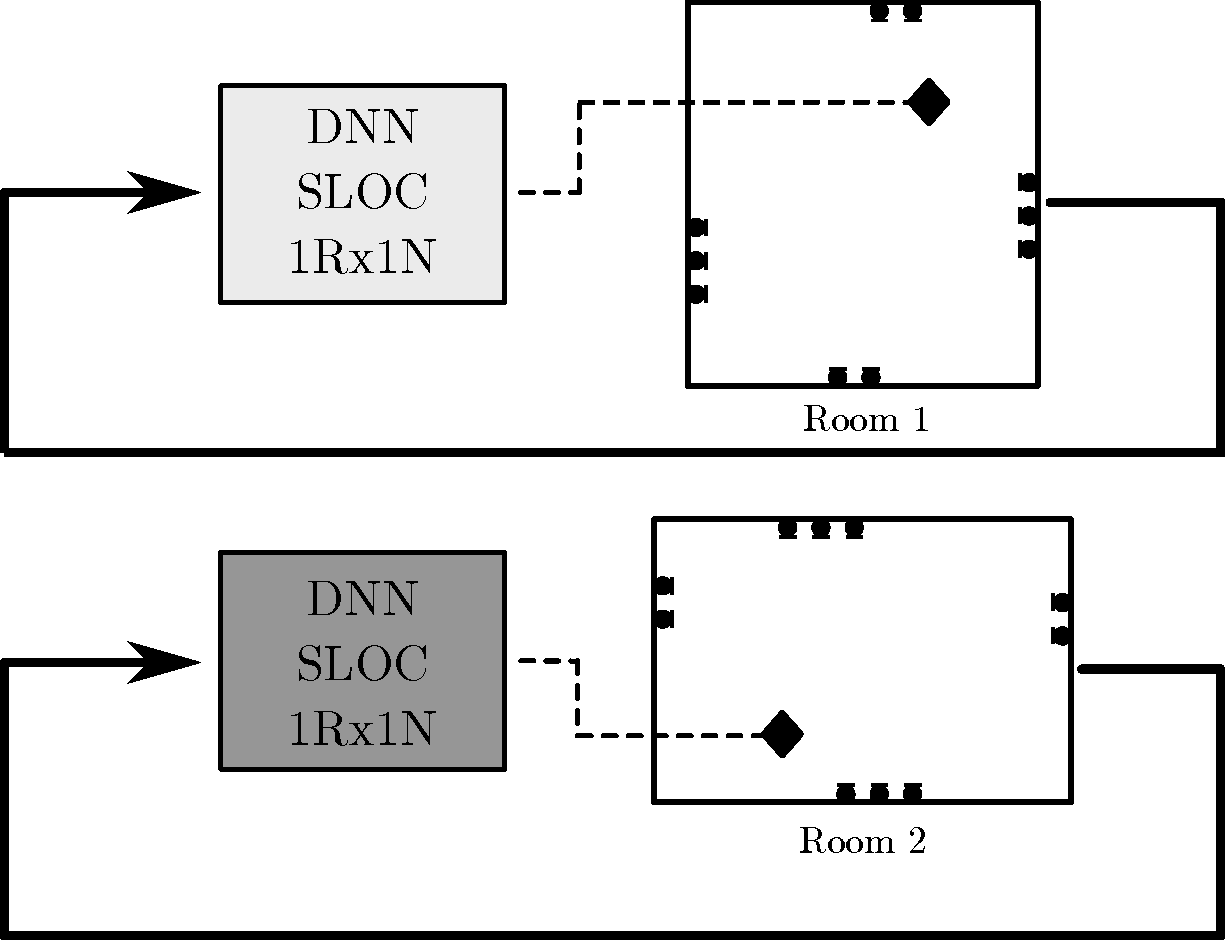
\includegraphics[width=\textwidth]{imgs/1Nx1R}\caption{}
	\end{subfigure}
	\hfill
	\begin{subfigure}[b]{0.45\textwidth}
	\centering
	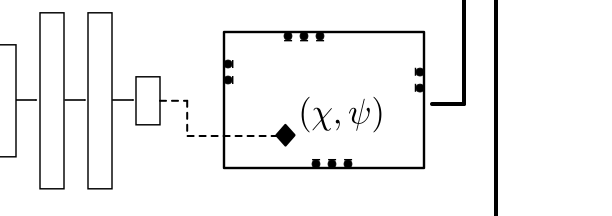
\includegraphics[width=\textwidth]{imgs/2Nx1R_3}\caption{}
  \end{subfigure}
	\caption{Block diagram of the proposed approach in a two-rooms scenario. The left side shows the diagram of the 1Rx1N-SLOC architecture, and the right side the diagram of the 2Rx1N-SLOC architecture. In the latter, both the DNN-SLOC algorithms localize the speaker in a single room by jointly exploiting the audio coming from both rooms.}
	\label{fig:2Rx1R}
\end{figure}


\subsection{Features based on GCC-PHAT Patterns}
\label{sec:features}

Processing several pairs of audio signals allows to identify the direction from which the signal arrives to the sensors, also called direction-of-arrival. By exploiting this information, it is possible to obtain the position of the speaker in a room. 

Due to sound wave propagation, a delay $\tau$ is expected between the source and a generic microphone. Considering two different microphones $a$ and $b$, it is possible to estimate the time difference $\Delta\tau_{ab} = \tau_a -\tau_b$ by using the Crosspower Spectrum Phase - Coherence Measure (CSPCM) \cite{knapp1976generalized}. %(\textbf{ndemap: non e' chiaro cosa c'entri la CSPCM con quello che viene scritto dopo}). 
%The computation of the GCC-PHAT is used in the TDOA estimation:
This method has the GCC-PHAT computation as a starting point:

\begin{equation}
\label{eq:CSPCM}
C_{ab}(n,\tau) =  \int_{-\infty}^{+\infty}{\frac{S_a(f,n) S_b^*(f,n)}{|S_a(f,n)| |S_b(f,n)|} \cdot e^{j2 \pi f \tau} df },
\end{equation}
where $S_a(f,n)$ is the Short-Time Fourier Transform of the frame $n$ of the signal $s_a(t)$ coming from a generic microphone. The TDOA is estimated as:
\begin{equation}\label{eq:tdoa}
\Delta\tau_{ab} = \underset{\tau}{\arg \max}\, C_{ab}(n,\tau).
\end{equation}
Successively, it is possible to calculate the DOA of the sound event for each microphone pair. 

In good acoustic conditions, with low reverberation time and sufficiently high SNR, this method gives an adequate DOA estimation \cite{zhang2008Phat}.
Nevertheless, due the numerous reflective surfaces and the variety of noises present in a multi-room domestic scenario these conditions are usually not satisfied.

Regarding to the proposed approach, preliminary experiments demonstrated that the simple TDOA estimation is not sufficiently reliable as input feature, thus we make use of GCC-PHAT Patterns, which have been previously employed in \cite{xiao2015learning}.
%Therefore the use GCC-Patterns compared to the TDOAs is more reliable and contains all the information required for the localization, so they are used as input features for the Neural Network \cite{xiao2015learning}. 

GCC-PHAT Patterns are calculated by using only microphone pairs belonging to the same array. Here, we suppose that the maximum distance $d_{max}$ between two sensors is equal to  50\,cm and that the sample rate $f_s$ is equal to 16\,kHz. Thus, the maximum time delay (in samples) between 2 microphones is:
\begin{equation}
\label{eq:TOA}
\Delta\tau_{max} = \frac{d_{max}}{\nu} \cdot f_s \approx 24,
\end{equation} 
where $\nu=340$\,m/s is the sound speed.
Hence, the GCC-PHAT Patterns are extracted as follows: for each considered microphone pair the CSPCM is computed with a \textcolor{red}{frame size equal to 30\,ms and a hop size equal to 10\,ms, corresponding to 480 samples and 160 samples at the sample rate of 16\,kHz.} %ndFAB
Under such conditions, only the central $2\Delta\tau_{max} + 1$ CSPCM values contain useful information. Thus, the first 50 values of $C_{ab}(n,\tau)$ are selected to compose the GCC-PHAT Pattern $\mathbf{x}_{ab}[n]$. 
Finally, the vectors originated by the different considered microphone pairs are standardized to have zero mean and unitary standard deviation.
Formally: 
\begin{align}
\mathbf{x}_{ab}[n] = & \;  [C_{ab}(n,0)\,C_{ab}(n,1) \cdots C_{ab}(n,49)]^T,\\
\tilde{\mathbf{x}}_{ab}[n] =  & \;  \frac{\mathbf{x}_{ab}[n] - \mu}{\sigma}, \label{eq:gcc_pattern}
\end{align}
where $\mu$ is the mean value of $\mathbf{x}_{ab}$, $\sigma$ the standard deviation, and $T$ denotes the transpose operation.

Successively, all possible combinations for each array are considered. In particular, the feature matrix related to the array $i$ composed of $N^{(i)}$ microphones assumes the following form:

\begin{equation}
\mathbf{X}^{(i)}[n] =   \begin{bmatrix} \tilde{\mathbf{x}}_{12}^{(i)}[n] \\ \tilde{\mathbf{x}}_{13}^{(i)}[n] \\ \vdots\\ \tilde{\mathbf{x}}_{1N^{(i)}}^{(i)}[n] \\ \tilde{\mathbf{x}}_{23}^{(i)}[n] \\\vdots \\ \tilde{\mathbf{x}}_{2N^{(i)}}^{(i)}[n] \\ \vdots \\  \tilde{\mathbf{x}}_{(N^{(i)}-1)N^{(i)}}^{(i)}[n] \end{bmatrix}.
\end{equation}

Finally, considering all the $M$ arrays located in the environment, the input matrix $\mathbf{X}[n]$ is given by:
\begin{equation}\label{eq:fx_matrix}
\mathbf{X}[n] =   \begin{bmatrix} \mathbf{X}^{(1)}[n] \\ \mathbf{X}^{(2)}[n] \\ \vdots\\ \mathbf{X}^{(M)}[n] \end{bmatrix},
\end{equation}
An example of $\mathbf{X}[n]$ is shown in \figref{fig:GCC-PATT}, where colors represent the amplitude of $C_{ab}(n,\tau)$, and orange tones denote the lowest values and blue tones the highest values in the range of $\tau$ considered. In the exposed case, the matrix $\mathbf{X}[n]$ is composed of 10 GCC-PHAT Patterns, belonging to a subset of the possible pairs originated from a circular ceiling array. It is possible to note that the maximum arrival time difference is equal to 9 samples (corresponding to about 0.2\,s), observed in the GCC-PHAT Pattern of the fourth microphone pair.


\begin{figure}[h]
	\centering
	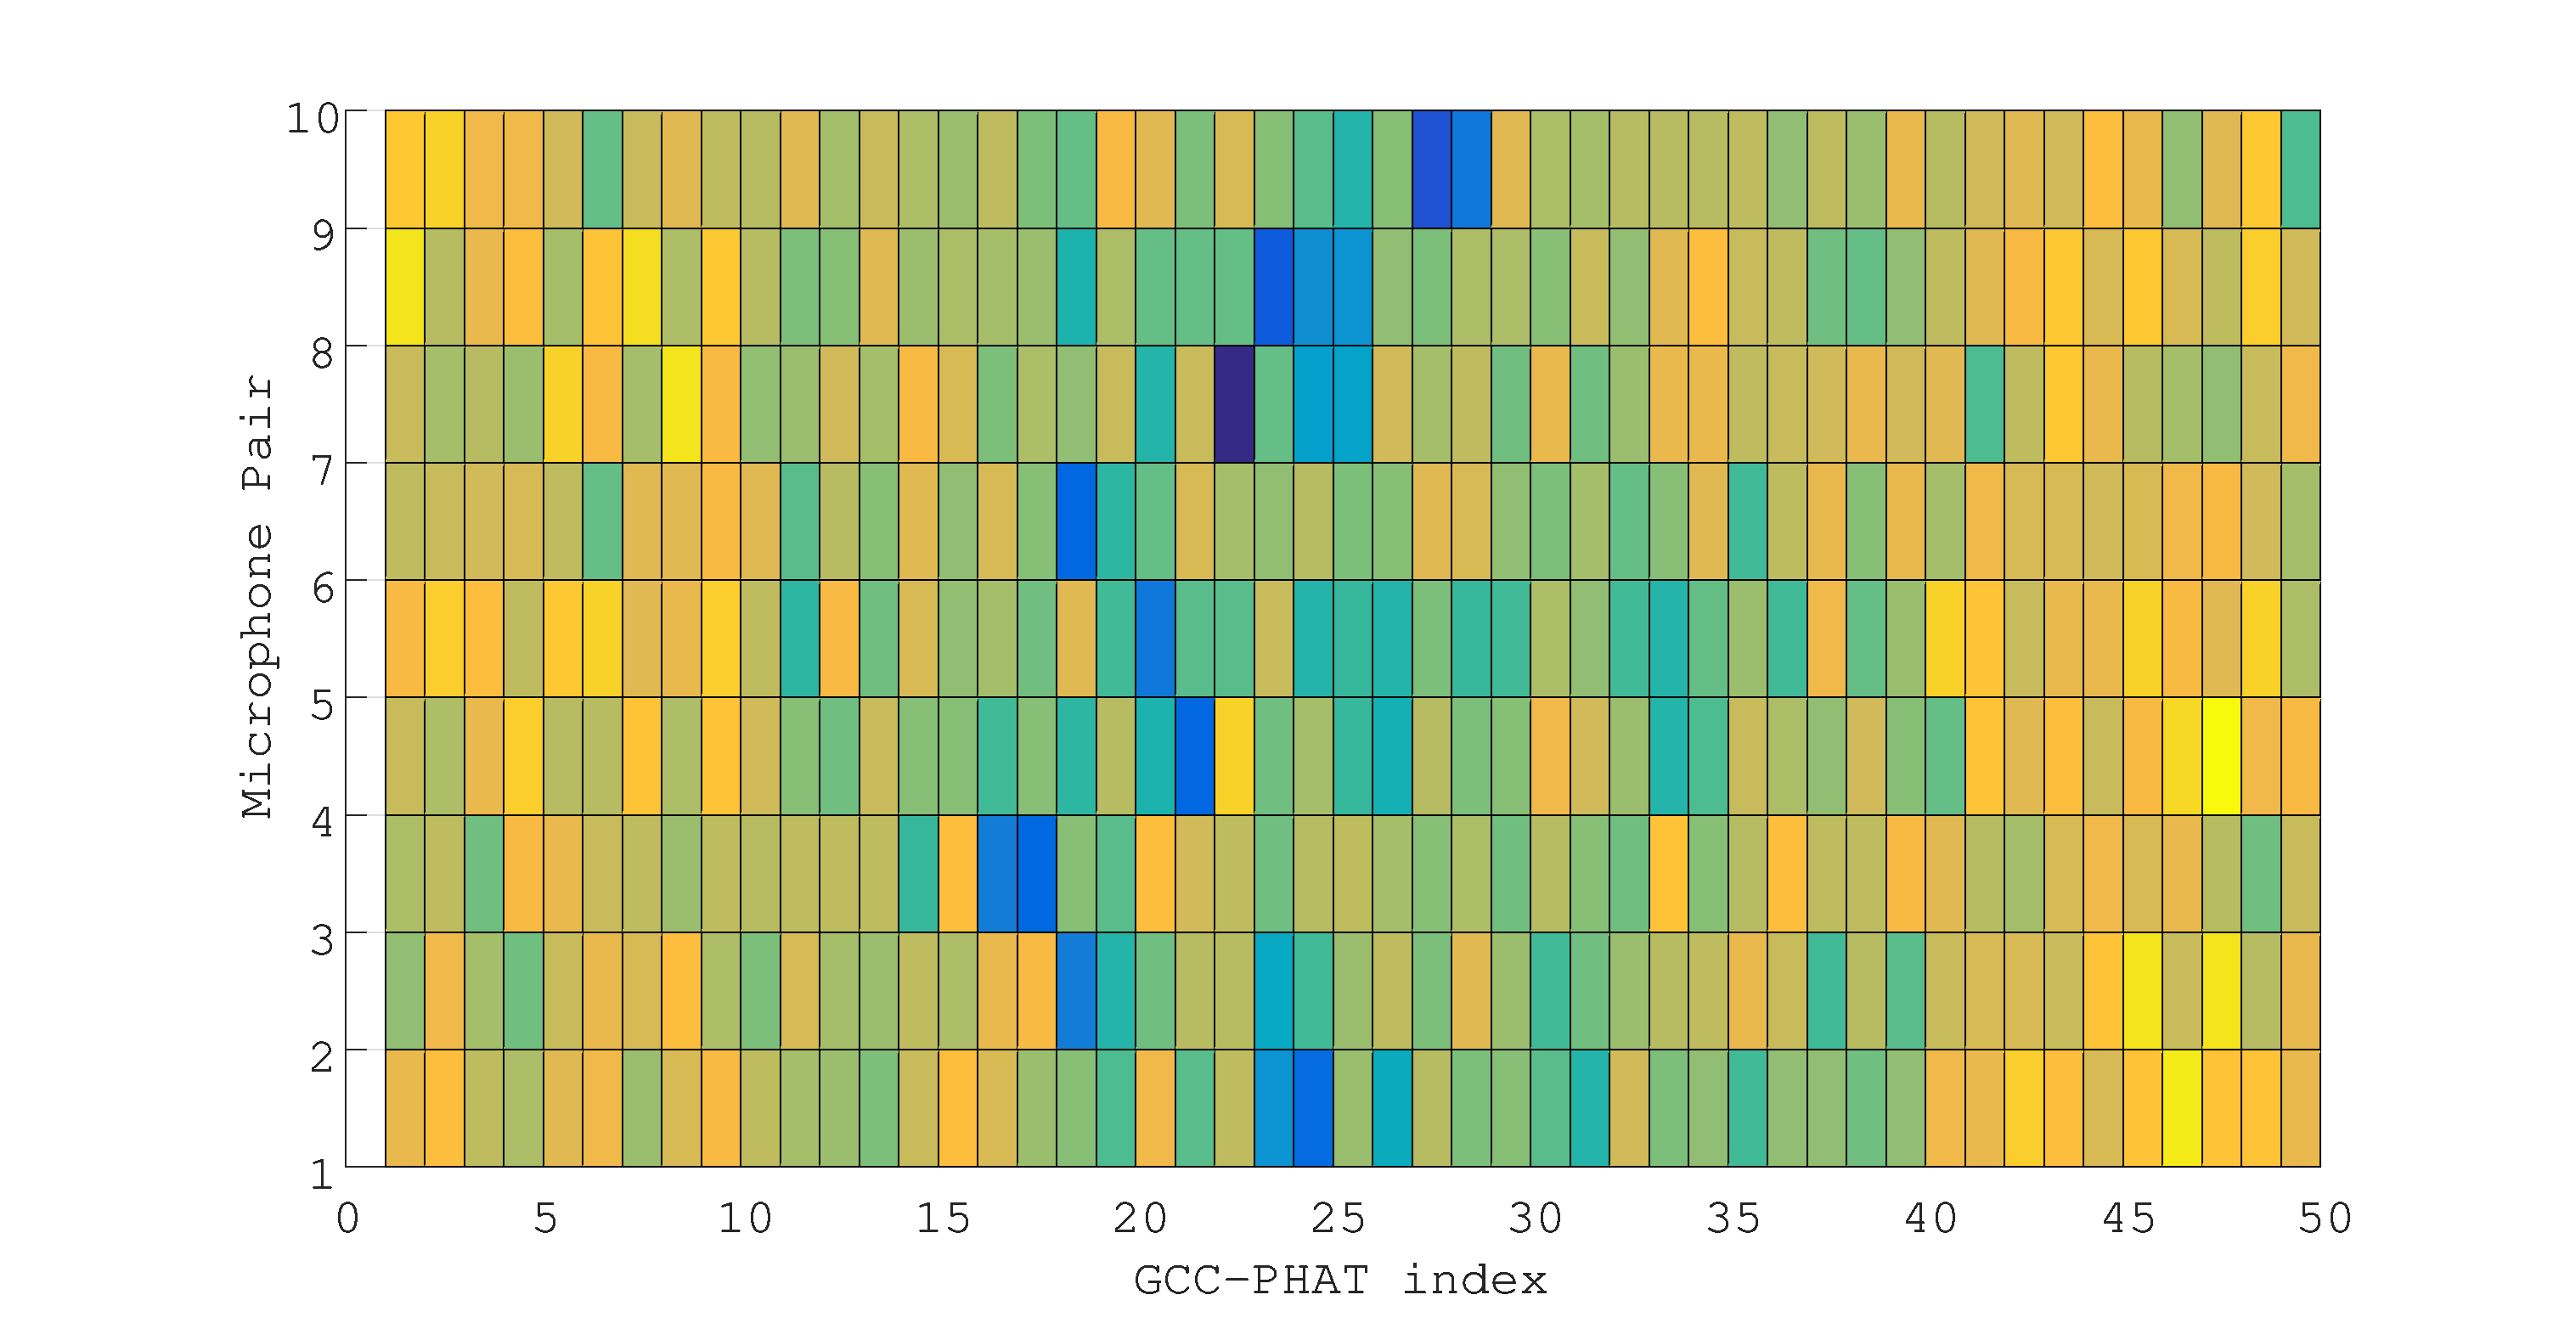
\includegraphics[width=0.9\columnwidth]{imgs/GCC-PHAT-PATTERN}
	\caption{An example of GCC-PHAT Pattern matrix $\mathbf{X}[n]$ obtained from a combination of microphones belonging to a ceiling array. Blue tones represent maximum amplitude values of $C_{ab}(n,\tau)$ in the range of considered $\tau$.}
	\label{fig:GCC-PATT}
\end{figure}

\subsection{Temporal Context}\label{sec:TEE}
The temporal context consists in the frames of the signal adjacent to the one being processed. In order to exploit this information, the input of the neural network  is augmented with $(C-1)/2$ GCC-PHAT Patterns preceding and following the current GCC-PHAT Pattern matrix $\mathbf{X}[n]$. The network, thus, estimates the speaker position by employing a \textit{chunk} of feature matrices defined as follows:

\begin{equation}
\overline{\overline{\mathbf{X}}}[n]= \left [ \begin{array}{c} 
\mathbf{X}[n -  \frac{C-1}{2} \cdot s]\\
\vdots\\
\mathbf{X}[n - s]\\
\mathbf{X}[n]\\
\mathbf{X}[n+s]\\
\vdots\\
\mathbf{X}[n + \frac{C-1}{2} \cdot s]
\end{array}
\right ],
\end{equation}
where $C$ is the total length of the chunk, and $s$ denotes the stride, which defines the extension of the chunk.  \textcolor{red}{The total length of the chunk in seconds is calculated as $\left [s\cdot H \cdot(C-1)+L \right ]/f_s$, where $H$ is the hop size in samples, and $L$ is the analysis frame length in samples.} \figref{fig:cxt_str} shows an example with $s=2$.

In cases where the selected frames do not contain speech, the GCC-PHAT Patterns matrices related to the first or the last frame of the segment are replicated accordingly.
%TODO sostituire ''do not contain speech'' con va fuori limite or similar...cf punto 6d dell Results discussion review

\begin{figure}[h] 
	\centering
	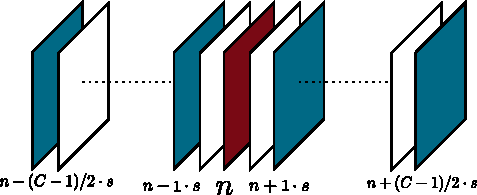
\includegraphics[width=0.65\columnwidth]{imgs/cxt_str}
	\caption{A scheme showing the GCC-PHAT Patterns matrices composing the temporal context. The GCC-PHAT Patterns matrix of current frame $\mathbf{X}[n]$ is shown in red ,the matrices included in the final chunk are shown in blue while the white matrices are those not considered as a result of the stride. The value of the stride $s$ is 2.}
		%(\textbf{ndemap: quelle bianche?})		
	\label{fig:cxt_str}
\end{figure} 

\subsection{Multi Layer Perceptron Neural Network}
\label{sec:MLP}
The first neural network architecture we investigate in this paper is the MLP \cite{Rumelhart86-LRB}. Indeed, it is well known that an  MLP with one or more hidden layers and a sufficient number of non-linear units (neurons) can  approximate any continuous  function  on  a  compact  input  domain  with arbitrary precision. For this reason, MLPs are said to be universal function approximators \cite{hornik1989multilayer}. A single neuron can be formally described as:
\begin{equation}
g(\mathbf{u}[n])=\varphi \left(\left(\begin{matrix} \sum _{ j=1 }^{ D }{w_j u_j[n] }  \end{matrix} \right) + b\right),
\end{equation}
where $D$ is the size of input data $\mathbf{u}[n]$, the bias $b$ is an externally applied term and $\varphi(\cdot)$ is the non-linear activation function. In this case we employ the ReLUs \cite{nair2010rectified}, defined as $\varphi(x) = \text{max}(0,x)$.
Thus, the mathematical description of a one-hidden-layer MLP is a function $f:\mathbb{R}^D \rightarrow \mathbb{R}^L$, where $L$ is the size of the output vector, so:

\begin{equation}
f(\mathbf{u}[n]) = 	\varphi \left( b_2 + W_2 \left( \varphi \left( b_1 + W_2 \cdot \mathbf{u}[n]\right) \right) \right),
\end{equation}
where $W_i$ and $b_{i}$ are the respective synaptic weights and the biases of the $i$-th layer.
The  behavior  of  this architecture  is  parametrized  by  the connection weights, which are adapted during the supervised network training, accomplished by using the Adam algorithm \cite{kingma2014adam} for the stochastic gradient-based optimization and a feature wise batch normalization \cite{ioffe2015batch}.

In the feature extraction block the GCC-PHAT Patterns are arranged in 2-D or 3-D matrices, whilst the MLP accepts input data as frame-by-frame vectors. \textcolor{red}{Thus, the matrices are flattened in a vector and the input layer consists of a number of units equal to $50 \cdot R\cdot C$, where $R$ is the number of rows of matrix $\mathbf{X}[n]$ defined in \eqref{eq:fx_matrix}.}

\textcolor{red}{Regarding the computational complexity, without taking into account the calculation of the GCC-PHAT Patterns  and considering additions and multiplications as separate operations \cite{DoSY07}, the total number of operations for each layer is given by 
\begin{equation}
\text{Cost}_{\text{MLP}} = \sum_{i=1}^P 2Q_{i-1}Q_i + \sum_{i=1}^{P-1} Q_i ,
\end{equation}
where $P$ is the number of layers, and $Q_i$ denotes the number of units of layer $i$. The first term, considers the number of operations for a linear unit, while the second term considers the operations required by the ReLU activation function. The upper bound of the second summation is $P-1$ since the last layer uses a linear activation function.
}

\textcolor{red}{Regarding the computational complexity, without taking into account the calculation of the GCC-PHAT Patterns  and considering additions and multiplications as separate operations \cite{DoSY07}, the total number of operations for each layer is given by 
\begin{equation}
\text{Cost}_{\text{MLP}} = \sum_{i=1}^P 2Q_{i-1}Q_i + \sum_{i=1}^{P-1} Q_i ,
\end{equation}
where $P$ is the number of layers, and $Q_i$ denotes the number of units of layer $i$. The first term, considers the number of operations for a linear unit, while the second term considers the operations required by the ReLU activation function. The upper bound of the second summation is $P-1$ since the last layer uses a linear activation function.
}


\subsection{Convolutional Neural Network}
\label{sec:CNN}
The birth of this kind of feed-forward neural network is related to image processing \cite{lawrence1997face}. Indeed, neural networks as MLPs take vectors as input, while this condition is not satisfied in the image case. The problem is tackled by means of convolutional layers, whose aim is to process restricted a area of a 2-D input, similarly to what happens in the animal visual cortex.
% Inspired by the animal visual cortex, CNN employs convolutional layers elaborating restricted area of a 2-D input. 
As in that case, the whole input matrix is processed by repeated application of a function across its sub-regions, obtaining so-called \textit{feature maps}. Practically, this is implemented by a convolution of the input data with a linear filter, adding a bias term and then applying a non-linear function.

Denoting the $m$-th feature map at a given $i$-layer as $h_{m,i}$, the $m$-th filter or \textit{kernel} is determined by the weights $W_{m,i}$ and bias $b_{m,i}$, thus:

\begin{equation}
h_{m,i}=\varphi	\left((W_{m,i} \ast \mathbf{u}_j[n]) + b_{m,i} \right),
\end{equation}
where $\ast$ represent the convolution operation.
The different feature maps obtained from each kernel of a convolutional layer are then summed to compose 
the input data for the following layer.

Commonly, a kernel layer is coupled with a pooling layer in order to assess more robustness against patterns shifts in the processed data. The CNN structure is completed by an MLP layer, whose task is to produce the network response, \textcolor{red}{i.e., the estimated $\left ( \chi,\psi \right ) $ positions in millimeters in this case.} %ndFAB

Although this architecture was designed for image processing, several works in the literature have employed CNNs in the audio field \cite{thomas2014analyzing,mcloughlin2015low}. In this work, we exploit a 3-D arrangement of the input data (as described in \secref{sec:TEE}), %(\textbf{ndemap: dove?})),
inspired by what occurs in image processing with RGB channels. Thus, the CNN-SLOC is able to efficiently process adjacent frames and to exploit the temporal evolution of the audio signal \cite{wirn2016-vad}. Up to the authors' knowledge, employing CNNs for indoor speaker localization are not present in the scientific literature.

According to that, the network first convolutional layer could respectively have 2-D or 3-D kernels: when a context size $C > 1$ is considered, the input features are organized in a 3-D tensor where the third axis represents the temporal index (as shown in \figref{fig:cxt_str}). In the degenerate case where $C$ is equal to 1, the tensor reduces to a bi-dimensional matrix.


\section{Comparative Methods}
\label{sec:comp_meth}
The proposed localization algorithm has been compared with two state-of-the art methods described in the remainder of this section.

\subsection{Crosspower Spectrum Phase Speaker Localization}\label{sec:soa_met}
The first algorithm taken as reference is the Crosspower Spectrum Phase speaker localization algorithm (CSP-SLOC) \cite{tsiami2014experiments}. \textcolor{red}{CSP-SLOC supposes that microphones and sources lie on the same plane, and it operates by calculating the intersection points of the DOA curves obtained from each pair of microphones. Ideally, all the curves should intersect at the same point, but since in reality this does not happen, a Maximum Likelihood obtained minimizing a least squares error criterion is performed. Tsiami \textit{et al.} \cite{tsiami2014experiments} improved the robustness of the estimate by pre-processing the microphone signals with a cepstral dereverberation algorithm  and by eliminating possible outliers.}

\textcolor{red}{More in details, the algorithm is evaluated separately for each room. Considering a set of microphone pairs, the first step consists in 
estimating the DOA angle ($\theta$) from the TDOA defined in \eqref{eq:tdoa} and the CSPCM defined in \eqref{eq:CSPCM}:}
\begin{equation}
\frac{d \cos \theta}{\nu} = \Delta\tau_{ab}  \Rightarrow \theta = \cos^{-1}  \left( \frac{\nu \Delta\tau_{ab} }{d} \right), 
\end{equation}
where $d$ is the distance between the microphones.

\textcolor{red}{After that, a Least Square algorithm is applied for resolving the ambiguity deriving from multiple intersection points of the DOA lines.  Considering, a random point $\mathbf{p}$ and its projection on the $j$-th DOA line $\mathbf{p}_{proj_j}$, the position $\hat{\mathbf{p}}$ is obtained by minimizing the error defined as the sum of the squared distances $D^2_j(\mathbf{p}) = \|\mathbf{p}-\mathbf{p}_{proj_j}\|^2$ between $\mathbf{p}$ and the $j$-th DOA:}
\begin{align}
E(\mathbf{p}) &= \sum_{j=1}^M D^2_j (\mathbf{p}),\\
\hat{\mathbf{p}} & =  \underset{\mathbf{p}} {\arg \min} \,E(\mathbf{p}), 
\end{align}
where $M$ is the number of DOA lines.

Several physical aspects affect the accuracy of the CSP-SLOC, such as the orientation of the speaker, the noise level and reverberation. In order to increase CSP-SLOC performance, the authors in \cite{tsiami2014experiments} adopted the pre-processing cepstral filtering technique described in \cite{stephenne1997new}. 

In this paper, the cepstral dereverberation algorithm uses frames of 2048 samples without overlap, with an exponential window having a scaling factor $\alpha = 0.9985$ and an averaging weighting coefficient $\mu=10^{-4}$. To be coherent with the proposed method, we computed the TDOAs with a rate of 100 frames/second and a frame overlap equal to 66\%.


\subsection{Steered Response Power Using the Phase Transform}
Another state of the art algorithm has been considered for comparison purpose. It consists in a modification of the Steered Response Power (SRP) method, based on the stochastic region contraction (SRC) approach, as described in \cite{DoSY07}. SRC avoids the complete fine grid-search, by applying an iterative process that progressively contracts the search volume for local maxima, thus reducing the overall computational cost.

As first step, a delay-and-sum beamformer is steered in the considered volume for each $n$-th frame of length $T$, leading to the SRP function for the spatial vector $\mathbf{s}$:

\begin{equation}
\label{eq:SRP}
P_n(\mathbf{s}) \equiv \int_{nT}^{(n+1)T} \left| \sum_{a=1}^M w_a s_a (t -\tau (\mathbf{s},a))\right|^2 dt,
\end{equation}
where $s_a(t)$ is the signal from a generic microphone $a$, $w_a$ its weight, $\tau (\mathbf{s},a)$ the distance in the time domain between $\mathbf{s}$ and that microphone. Practically, \eqref{eq:SRP} is evaluated in the frequency domain, scaled by the phase transform weighting factor (PHAT). The SRC is iteratively applied: $J_0 = 5000$ points are randomly evaluated, $N_0 = 20$ points maximizing \eqref{eq:SRP} are selected and the search volume is restricted to a smaller region that contains the $N_0$ points. In the following, this algorithm will be referred as SRP-SLOC.




\section{The DIRHA Dataset}
\label{sec:dataset}

\begin{figure}[h]
	\centering
	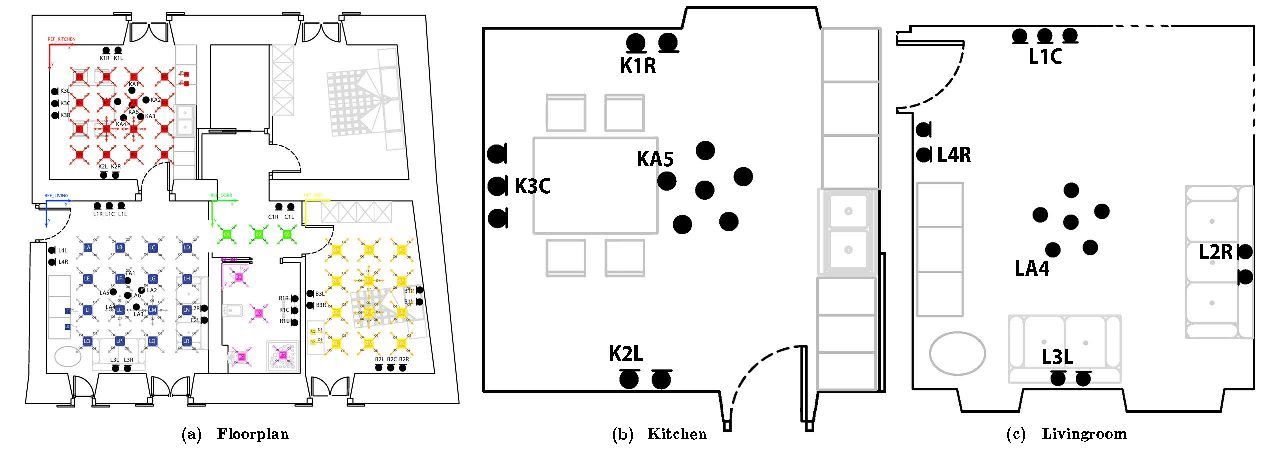
\includegraphics[width=\textwidth]{imgs/plan}
	\caption{The map of the apartment used for the DIRHA project (a). Figures (b) and (c) show the considered rooms, with the disposition of their relative microphones. }
	\label{fig:DIRHA_map}
\end{figure}

The analysis of the DNN-SLOC performance has been conducted on the DIRHA dataset \cite{cristoforetti2014dirha}, characterized by diverse scenes, rooms, microphones and noise conditions\footnote{\url{http://dirha.fbk.eu/simcorpora}}. In details, the apartment where the dataset has been recorded consists in five rooms and a total of 40 microphones. These are arranged in linear and circular arrays, with the first ones placed on the walls of all rooms, and the circular ones are placed on the ceiling of the living room and of the kitchen (\figref{fig:DIRHA_map}).

The dataset is composed of two subsets, named \emph{Simulated} and \emph{Real}. For each of them several \textit{scenes} have been recorded, composed of typical situations observable in a domestic context. As reported in \tableref{tab:dataset}, the two subsets differ in terms of scenes and total length: in the Simulated set the scenes length is fixed to 60 seconds, while it varies in the Real set. In addition, the latter has been recorded with persons moving in the rooms and speaking towards different directions throughout the scenes, whilst the Simulated has been obtained by convolving a fixed set of measured Room Impulse Responses (RIRs) with recorded signals.
The Simulated subset is also characterized by a lower SNR compared to the Real one and overlapping speech does not occur.

Our study focuses on two rooms of the dataset, i.e.,  the Kitchen and the Living Room, due to three main aspects. First of all, these rooms consist in the area of a home-environment where most of the events take place. In addition, being the widest rooms of the apartment, the localization task is more challenging. \textcolor{red}{The room dimensions are respectively $4790 \times 3800\, \left [mm\right ]$ for the Kitchen and $4790 \times 4850\, \left [mm\right ]$ for the Living Room.}
Finally, the number of microphones are higher compared to the other rooms, and it comprises both wall and ceiling arrays.

\begin{table}[t]
	%\renewcommand{\arraystretch}{1.2}
	\centering
%	\small
	\caption{Main differences between the Real and Simulated subsets.}
	\resizebox{.75\columnwidth}{!}{%
	\begin{tabular}{c|c|c}\hline
		& \textbf{Real} & \textbf{Simulated} \\ \hline
		\textbf{Nr.\ of Scenes}  & 22 & 80 \\ \hline
		
		\textbf{Total Duration} &  21.5 min. & 80 min.  \\  \hline
		\multirow{2}{*}{\textbf{Speech Percentage}}	&  12.9\%  & 23.6\%  \\
		& 	2.8  min.	& 18.9 min. \\ \hline
		\textbf{Source} & human (moving) & loudspeaker (static) \\ \hline
		\textbf{Background} & quiet & various \\ \hline
		\textbf{Noise Source Rate} & low & high \\ \hline
		\textbf{Overlapping Events} & no & yes \\ \hline  
	\end{tabular} 
	}
	\label{tab:dataset}
\end{table}


\section{Experiments}
\label{sec:expRes}
In this section the experimental procedure is presented and the obtained results are discussed. 

\subsection{Experimental setup}
The performance of the two proposed methods, 1Rx1N-SLOC and 2Rx1N-SLOC described in \secref{sec:ALGO}, are investigated in the two DIRHA subsets.
Both architectures have been evaluated by using MLP and CNN. The experiments have been performed by assuming the presence of an Oracle multi-room Voice Activity Detector (VAD), which selects only the speech portions of the audio signals.

The experiments have been conducted by means of a $k$-fold cross-validation technique in order to reduce the performance variance, and an early-stopping training strategy has been employed to prevent overfitting. In the \textit{Simulated} dataset $k$ is equal to 10, thus 64-8-8 scenes respectively compose the training, validation and test sets. In the \textit{Real} dataset, due to the total absence of speech in some scenes, only 11 of them were suitable for each room. Thus, a leave-2-out cross validation has been adopted, where 7 scenes compose the training set, 2 the validation set and 2 the test set.

The selection of the most performing DNN-SLOC architecture has been carried out by means of a four-stage optimization strategy, described as follow:

\begin{enumerate}
	\item{\textbf{Network Size Selection.}}  It consists in varying the network layout while keeping fixed the input signals (i.e., 4 microphone pairs for the Kitchen and 5 microphone pairs for the Living Room). 
	Concerning the MLP architecture, 30 different network topologies have been investigated, composed of 1, 2 or 3 hidden layers with 4, 8, \dots, 1024 units. 
	On the contrary, in the case of CNN architecture a higher number of parameters must be considered, which have been reported in \tableref{tab:CNNs} for the sake of conciseness. 
	\item{\textbf{GCC-PHAT Patterns Selection.}} \textcolor{red}{The objective of this stage is to find the composition of the feature matrix $\mathbf{X}[n]$ defined in \eqref{eq:fx_matrix} that provides the best localization performance. The procedure is performed separately for each room and it starts by considering the circular arrays on the ceilings: each array is composed of 6 microphones, thus, excluding the central one, the number of microphone pairs is 10 and the size of the initial feature matrix is $10 \times 50$. This matrix is then augmented by gradually including the GCC-PHAT Patterns $\mathbf{\tilde{x}}_{ab}[n]$ (see \eqref{eq:gcc_pattern}) related to the pairs of microphones of the remaining arrays of the room. If the inclusion of the GCC-PHAT Pattern results in a performance improvement, it is retained, otherwise it is discarded.}
	
%	This stage aims to find the most performing GCC-PHAT Patterns matrix $\mathbf{X}[n]$ between a subset of the available $\mathbf{X}^{(i)}[n]$ microphone combinations belonging to different arrays.
%	The starting point was the circular array placed on the room ceilings, which is composed of $N = 6$ microphones. Excluding the central one, it leads to 10 possible pairs. Then, combinations of signal pairs $\mathbf{\tilde{x}}_{ab}^{(i)}[n]$ coming from the wall arrays have been gradually added to the ceiling array signals with a sequential forward selection strategy, in order to arrange the evaluated $\mathbf{X}[n]$.
	%TODO cf. punto 6e) modifiche al testo
	\item{\textbf{Network Size Selection.}} Another network size selection is then performed, having as input features the set of GCC-PHAT Patterns providing the best results in the previous step. 
	\item{\textbf{Temporal Context Selection.}} Here the objective is evaluating the effects of the temporal context, by varying the strides values, i.e., $s=\{1,3,4,5\}$, and the context dimensions, i.e., $C=\{3,7,11,13,15,17,19,21\}$.
\end{enumerate}


\begin{table}[t]
	\centering
	%\setlength{\tabcolsep}{2.pt}
	\small
	%\renewcommand{\arraystretch}{1.1}
	\caption{Network topology parameter explored during the optimization stages.}
	\label{tab:CNNs}
	\resizebox{.8\columnwidth}{!}{%
	\begin{tabular} { c|c|c|c|c|c|c|c}
		\hline
		\multicolumn{8}{c}{CNN}\\
		\hline
		\multicolumn{3}{c|}{\begin{tabular}[c]{@{}c@{}}First \\ Convolutional \\ Layer\end{tabular}}                                                                                                                                            & \multicolumn{3}{c|}{\begin{tabular}[c]{@{}c@{}}Second\\ Convolutional\\ Layer\end{tabular}}                                & \multicolumn{2}{c}{Neurons}                                                                                                                             \\ \hline
		\begin{tabular}[c]{@{}c@{}}Nr.\ of\\ Kernels\end{tabular}          & Size                                                                                 & Pooling                                                                   & \begin{tabular}[c]{@{}c@{}}Nr.\ of\\ Kernels\end{tabular}           & Size                          & Pooling            & \begin{tabular}[c]{@{}c@{}}I \\ Layer\end{tabular}                        & \begin{tabular}[c]{@{}c@{}}II \\ Layer\end{tabular}                  \\ \hline
		\multirow{4}{*}{\begin{tabular}[c]{@{}c@{}}16\\ 24\\ 48\end{tabular}} & \multirow{4}{*}{\begin{tabular}[c]{@{}c@{}}3 $\times$ 3\\ 5 $\times$ 5\end{tabular}} & \multirow{4}{*}{\begin{tabular}[c]{@{}c@{}}2 $\times$ 2\\ -\end{tabular}} & \multirow{4}{*}{\begin{tabular}[c]{@{}c@{}}16\\ 24\\ 48\end{tabular}} & \multirow{4}{*}{2 $\times$ 2} & \multirow{4}{*}{-} & \multirow{4}{*}{\begin{tabular}[c]{@{}c@{}}64\\ 128\\ 256\\ 512\end{tabular}} & \multirow{4}{*}{\begin{tabular}[c]{@{}c@{}}128\\ 256\\ 512\end{tabular}} \\
		&                                                                                      &                                                                           &                                                                       &                               &                    &                                                                               &                                                                          \\
		&                                                                                      &                                                                           &                                                                       &                               &                    &                                                                               &                                                                          \\
		&                                                                                      &                                                                           &                                                                       &                               &                    &                                                                               &                                                                          \\ \hline
		\hline
		\multicolumn{8}{c}{MLP}\\
		\hline
		Fully  & Nr.  & \multicolumn{3}{|c|}{4, 8, 16,} & Nr. &  \multicolumn{2}{|c}{ }\\
		Connected	& of & \multicolumn{3}{|c|}{32, 256,} & of & \multicolumn{2}{|c}{ 1, 2, 3}\\
		Layers	& Units & \multicolumn{3}{|c|}{512, 1024} & Layers & \multicolumn{2}{|c}{} \\
		\hline                                                                      
	\end{tabular}
	}
\end{table}


The localization accuracy has been evaluated in terms of averaged Root Mean Square Error (RMSE):
\begin{equation}
\text{RMSE} = \frac{\sqrt{(\chi-\chi_{\text{ref}})^2 + (\psi-\psi_{\text{ref}})^2}}{N_{TOT}},
\end{equation}
where $\chi$ and $\psi$  are the network outputs, $\chi_{\text{ref}}$ and $\psi_{\text{ref}}$ are the reference Cartesian coordinates, and $N_{TOT}$ is the total number of \textcolor{red}{speech} frames, \textcolor{red}{{as reported in \tableref{tab:N_TOT}. }}
In addition, the performance has been evaluated in terms of $P_{cor} = N_{FINE}/N_{TOT}$, where $N_{FINE}$ is the 
number of frames with RMSE less than 500\,mm. 
%%ndFAB
Similarly to a classification task, $P_{cor}$ provides a measure of the localization accuracy, since the estimated positions with an RMSE less than 500\,mm are considered correct decisions. \textcolor{red}{The performance metrics and the related hyperparameters have been chosen according to the guidelines of the Speech Activity detection and Speaker LOcalization in DOMestic environments (SASLODOM 2014)\footnote{http://dirha.fbk.eu/SASLODOM2014} task of the EVALITA 2014 challenge \cite{basili2014proceedings}.} These two metrics are averaged over all the available network outputs. 

\begin{table}[t]
\centering
\begin{tabular}{cccc}
\hline
\multicolumn{2}{c|}{\textbf{Simulated Dataset}} & \multicolumn{2}{c}{\textbf{Real Dataset}} \\ \hline
\multicolumn{1}{c|}{Kitchen}           & \multicolumn{1}{c|}{Livingroom}          & \multicolumn{1}{c|}{Kitchen}                  & Livingroom                  \\ \hline
\multicolumn{1}{c|}{47630}             & \multicolumn{1}{c|}{44801}               & \multicolumn{1}{c|}{17580}                    & 12885  \\
\hline                    
\end{tabular}
\caption{Number of speech frames ($N_{TOT}$) for the considered rooms of the two datasets.}\label{tab:N_TOT}
\end{table}

The algorithm has been implemented in the Python language using Keras \cite{chollet2015keras} and Theano \cite{2016arXiv160502688short} as deep learning libraries. A total amount of 2350 experiments has been conducted on the two subsets of the DIRHA dataset.

%The parameters of the training optimizer employed in the experiments are the following: 
%\begin{itemize}
%	\item weight initialization: gaussian distribution with $\mu=0$ and $\sigma=0.1$
%	\item training epochs: 200 with 50 epochs of patience and 500 with 50 epochs of patience respectively for CNN and MLP
%	\item learning rate: 0.025 for CNN and 0.001 for MLP.
%\end{itemize}
%Where not specified, the default parameters defined in Keras were used.

The parameters of the training optimizer (i.e., Adam, batch normalization \cite{kingma2014adam, ioffe2015batch}) are set as shown in \tableref{tab:training}.

\begin{table}[h]
	%\renewcommand{\arraystretch}{1.0}
	\caption{Parameters of the Adam optimizer selected for the neural network training. ``E.S.'' denotes early stopping strategy, evaluated on the validation loss.}
	\label{tab:training}
	\centering
	\resizebox{.82\columnwidth}{!}{%
		\begin{tabular}{l|cccc}
			\hline
			&  \textbf{Weight}  &  \multirow{2}{*}{\textbf{Epochs}} & \textbf{Optimizer} \\ 
			&  \textbf{initialization} & & \textbf{parameters}\\ 
			\hline
			\multirow{3}{*}{CNN}& Gaussian distr. & 200 & learn. rate = 0.025, \\
			& $\mu=0$  &     50 E.S. patience 	& $\beta_1=0.9$, $\beta_2=0.999$, \\
			& $\sigma=0.1$ & & $\epsilon=10^{-8}$ \\ 
			\hline
			\multirow{3}{*}{MLP}  & Gaussian distr. & 500 & learn. rate = 0.001, \\
			& $\mu=0$  &     50 E.S. patience  	& $\beta_1=0.9$, $\beta_2=0.999$, \\
			& $\sigma=0.1$ & & $\epsilon=10^{-8}$ \\ 		
			\hline
			\hline
			\multicolumn{4}{c}{\textbf{Batch Normalization:}  $\epsilon = 10^{-6}$, $\mu=0.9$}  \rule{0pt}{8pt} \\
			\hline
		\end{tabular}
	}
\end{table}




\subsection{Results on the Simulated Dataset}
\label{sec:exp_simu}


\begin{table}[!h]
	\centering
	\caption{Comparison of best results of SLOC algorithms in terms of RMSE (mm) and $P_{cor}$ (\%) in the Simulated case study. The temporal context is espressed in terms of $C$ - $s$ (frame), respectively the total length of the chunk and the stride.}
		%\textbf{ndemap: cosa vuole dire la colonna ``Context''? Ad es, 19-4: 19? 4?.}
		\label{tab:results_SIMU}
	%\renewcommand{\arraystretch}{1.1}
	\resizebox{\columnwidth}{!}{
	\begin{tabular}{l|ccc|ccc|cc}
		\hline \hline
		\multicolumn{9}{c}{SIMULATED}                                                                                                                                                                                                                          \\
		\hline
		ROOM      & \multicolumn{3}{c|}{Kitchen}                                                            & \multicolumn{3}{|c|}{Living Room}                                                        & \multicolumn{2}{c}{Average}                              \\
		\hline
		& \multicolumn{1}{l}{$C$ - $s$ (frame)} & \multicolumn{1}{r}{RMSE (mm)} & \multicolumn{1}{l|}{$P_{cor}$ (\%)} & \multicolumn{1}{l}{$C$ - $s$ (frame)} & \multicolumn{1}{l}{RMSE (mm)} & \multicolumn{1}{l|}{$P_{cor}$ (\%)} & \multicolumn{1}{l}{RMSE (mm)} & \multicolumn{1}{l}{$P_{cor}$ (\%)} \\
		\hline
		\hline
		
		MLP 1Rx1N & /                          & 475                      & 60                            & /                          & 575                      & 64                            & 525                      & 62                            \\
		MLP 1Rx1N & 19 - 4                      & 370                      & 69                            & 17 - 4                      & 442                      & 72                            & 406                      & 71                            \\ \hline
		MLP 2Rx1N & /                          & 453                      & 59                            & /                          & 571                      & 62                            & 512                      & 61                            \\
		MLP 2Rx1N & 17 - 3                      & 375                      & 67                            & 19 - 3                      & 455                      & 70                            & 415                      & 68                            \\ \hline
		CNN 1Rx1N & /                          & 529                      & 57                            & /                          & 625                      & 63                            & 577                      & 60                            \\
		CNN 1Rx1N & 21 - 4                      & 309                      & 75                            & 21 - 3                      & 358                      & 78                            & 333                      & 77                            \\ \hline
		CNN 2Rx1N & /                          & 522                      & 57                            & /                          & 635                      & 61                            & 579                      & 59                            \\
		CNN 2Rx1N & 21 - 4                      & 331                      & 73                            & 17 - 5                      & 374                      & 75                            & 353                      & 74                            \\ \hline
		CSP-SLOC  & /                          & 1281                     & 8                             & /                          & 1648                     & 8                             & 1464                     & 8                             \\ \hline
		SRP-SLOC  & /                          & 1005                     & 22                            & /                          & 958                      & 37                            & 981                      & 30 \\ 
	\end{tabular}
	}
\end{table}



\subsubsection{Evaluation without the temporal context}
The results obtained by the different addressed algorithms in the Simulated case study are reported in \tableref{tab:results_SIMU}, both with and without the temporal context (i.e., respectively at the end of the third and the fourth optimization stage).

Focusing on the performance obtained without temporal context, the best DNN configuration is the 2Rx1N MLP-SLOC. In particular, both int the 1Rx1N and  2Rx1N configurations, the MLP performs slightly better than the CNN. 
Furthermore, even if only little improvement is observable in terms of RMSE for the 2Rx1N case, the advantage of this setting lies in the statistical behavior, as reported in \figref{fig:boxplot_simu-mlp}. 
The boxplots show in terms of mean and standard deviation a narrow dispersion of results for both the CNN and MLP architectures.
%Indeed, by using the audio from both rooms reduces the dependence on the microphones location inside the room.
%ndFAB results discussion 6a) 
\textcolor{red}{{Indeed, by using the audio from both rooms reduces the dependence on the microphones location inside the room as it is proved by a reduced area between the mean plus variance and mean less variance values. In particular, in the case of the MLP there is also an absolute reduction of the error by comparing the minimum and maximum values of the RMSE.}}
%%
In details, the best MLP layouts for the Kitchen and Living room are two single layer networks of 256 and 1024 units, respectively. %As concerns the CNN-SLOC, the two best layouts are composed of a single convolutional layer of 48 kernels of size 5$\times$5 with no pooling, followed by a two layers MLP with  512, 512 units and 128, 256 units respectively for Kitchen and Living Room.
With regards to the CNN-SLOC, the two best layouts are the following: for the Kitchen, a single convolutional layer of 48 kernels of size 5$\times$5 with no pooling, followed by two feed-forward layers with 512, 512 units, while for Livingroom, a single convolutional layer of 24 kernels of size 5$\times$5 with no pooling, followed by two feed-forward layers with 256 and 512 units.

The CSP-SLOC and the SRP-SLOC algorithms obtain a lower localization performance compared to the neural network architectures, with an average RMSE respectively equal to 1464\,mm and 981\,mm.



\newenvironment{customlegend}[1][]{%
	\begingroup
	% inits/clears the lists (which might be populated from previous
	% axes):
	\csname pgfplots@init@cleared@structures\endcsname
	\pgfplotsset{#1}%
}{%
% draws the legend:
\csname pgfplots@createlegend\endcsname
\endgroup
}%

% makes \addlegendimage available (typically only available within an
% axis environment):
\def\addlegendimage{\csname pgfplots@addlegendimage\endcsname}

\begin{figure}[t]
	\centering
	\begin{tikzpicture}[scale=0.75]
	\begin{axis}[
	%legend entries = {1Rx1N, 2Rx1N},
	% legend to name={legend},
	title = Simulated Dataset - GCC SELECTION,
	boxplot/draw direction=y,
	x axis line style={opacity=0},
	axis x line*=bottom,
	axis y line=left,
	enlarge y limits,
	ymajorgrids,
	%xtick={1,3,5,7},
	%xticklabel style = {font=\tiny},
	xtick={1.5,3.5},
	xticklabels={CNN, MLP},
	ylabel={RMSE (\%)},
	ytick={},ymin=515,ymax=700]
	]
	%BLUE MLP
	%RED CNN
	\addplot+[
	boxplot prepared={
		median=618,
		upper quartile=634,
		lower quartile=602,
		upper whisker=661,
		lower whisker=564
	},fill=BoxCol,draw=BoxCol,fill opacity=0.8, 
	] coordinates {};
	%\addlegendentry{1Rx1N}
	\addplot+[
	boxplot prepared={
		median=621.5,
		upper quartile=631,
		lower quartile=612,
		upper whisker=695,
		lower whisker=584
	}, fill=BoxCol1,draw=BoxCol1,fill opacity=0.8
	] coordinates {};
	%\addlegendentry{2Rx1N}
	\addplot+[
	boxplot prepared={
		median=578.5,
		upper quartile=588,
		lower quartile=569,
		upper whisker=603,
		lower whisker=527
	}, fill=BoxCol,draw=BoxCol,fill opacity=0.8
	] coordinates {};
	\addplot+[
	boxplot prepared={
		median=559.5,
		upper quartile=567,
		lower quartile=552,
		upper whisker=595,
		lower whisker=523
	}, fill=BoxCol1,draw=BoxCol1,fill opacity=0.8
	] coordinates {};
	\end{axis}
	
	\begin{customlegend}[legend entries={1Rx1N, 2Rx1N}, legend style={at={(6.2,5.5)}} ]
	% \node (rel axis cs:0.9,0.2);
	
	\addlegendimage{BoxCol,fill=BoxCol,fill opacity=0.8,area legend}
	\addlegendimage{BoxCol1,fill=BoxCol1,fill opacity=0.8,area legend}
	\end{customlegend}
	
	\end{tikzpicture}
	\caption{Boxplot for the Simulated dataset, for MLP and CNN neural network, comparing 1Rx1N and 2Rx1N setups. This evaluation is performed at the end of the second stage of optimization, considering all the tested GCC Patterns configurations. The results are averaged over the two target rooms.}
	\label{fig:boxplot_simu-mlp}
\end{figure}

\begin{table}[!h]
	\centering
	\caption{Results for Convolutional Neural Networks with the best performing configurations in the Simulated case study.}
	\label{tab:bestCONF_SIMU}
	\resizebox{\textwidth}{!}{%
	\begin{tabular}{c|cc|cc|cc|cc|cc}
		%\cline{2-11}
		\multicolumn{1}{l|}{}        & \multicolumn{2}{c|}{Features Settings}                    & \multicolumn{2}{c|}{Microphones}                                                                   & \multicolumn{2}{c|}{\begin{tabular}[c]{@{}c@{}}Convolutional \\ Kernels\end{tabular}} & \multicolumn{2}{c|}{Feed Forward Layers}    & \multicolumn{2}{c}{Results}               \\ \hline
		\multirow{2}{*}{Room}        & \multirow{2}{*}{Configuration} & \multirow{2}{*}{ $C$ - $s$ (frames)} & \multicolumn{1}{c}{\multirow{2}{*}{Ceiling}}                              & \multirow{2}{*}{Wall} & \multirow{2}{*}{Number}                 & \multirow{2}{*}{Size}                       & First                & Second               & RMSE                 & $P_{cor}$           \\
		
		&                                &                          & \multicolumn{1}{c}{}                                                      &                       &                                         &                                             & Layer                & Layer                & (mm)                 & (\%)                \\ \hline
		\hline
		\multirow{3}{*}{Kitchen}     & \multirow{3}{*}{1Rx1N}         & \multirow{3}{*}{21 - 4}  & \multirow{3}{*}{\begin{tabular}[c]{@{}c@{}}Circular \\ Array\end{tabular}} & K3L,K3C               & \multirow{3}{*}{48}                     & \multirow{3}{*}{$5\times5$}                 & \multirow{3}{*}{512} & \multirow{3}{*}{512} & \multirow{3}{*}{309} & \multirow{3}{*}{75} \\
		&                                &                          &                                                                            & K2L,K2R               &                                         &                                             &                      &                      &                      &                     \\
		&                                &                          &                                                                            & K1R,K1L               &                                         &                                             &                      &                      &                      &                     \\ \hline
		\multirow{4}{*}{Living Room} & \multirow{4}{*}{1Rx1N}         & \multirow{4}{*}{21 - 3}  & \multirow{4}{*}{\begin{tabular}[c]{@{}c@{}}Circular \\ Array\end{tabular}} & L4L,L4R               & \multirow{4}{*}{24}                     & \multirow{4}{*}{$5\times5$}                 & \multirow{4}{*}{256} & \multirow{4}{*}{512} & \multirow{4}{*}{358} & \multirow{4}{*}{78} \\
		&                                &                          &                                                                            & L3L,L3R               &                                         &                                             &                      &                      &                      &                     \\
		&                                &                          &                                                                            & L2L,L2R               &                                         &                                             &                      &                      &                      &                     \\
		&                                &                          &                                                                            & L1R,L1C               &                                         &                                             &                      &                      &                      &                     \\
	\end{tabular}
	}
\end{table}



\subsubsection{Evaluation including the temporal context}
The effect of temporal context is considered in the final optimization stage, in which the network size determined after the third stage is kept fixed. %This last stage is compared to the previous in order to highlight the decisive effect of the exploitation of an audio excerpt.  

The best localization performance has been obtained by using the CNN-SLOC having as input the microphone signals coming only from the target room. The resulting averaged RMSE is equal to 333\,mm and the highest $P_{cor}$ is 77\%. The details of the configuration parameters for the best performing setups on the Simulated subset are shown in \tableref{tab:bestCONF_SIMU}. The performance improvement at this stage is evident, whereas the employment of multiple room audio features does not seem to have a beneficial effect for CNN based algorithms. 
%by the variation of the feature set, except as previously said about stability to vary of the input microphones. %(da modificare)

The results obtained at the very end of the optimization procedure show the ability of the CNN architecture to efficiently exploit the contextual information of adjacent frames, with a reduction of 42.2\% of the localization error with respect to the configuration with $(C,s)=(1,1)$, as shown in \figref{fig:cxtCNN-S}. 
The best resulting values of context and strides are $(C,s)=(21,4)$ and $(C,s)=(17,5)$ for Kitchen and Living Room, respectively, which means processing a segment of duration equal to \textcolor{red}{0.83\,s for both rooms.} 

\begin{figure}[t]
	\centering
	\begin{tikzpicture}[scale=0.8]
	\begin{axis}[
	ybar,
	bar width=23pt,
	x axis line style={opacity=0},
	axis x line*=bottom,
	axis y line=left,
	enlarge y limits,
	title style={at={(0.22,1.00)}},
	title = {Simulated Dataset - CNN-SLOC},
	ymajorgrids,
	xticklabel style={align=center}, xticklabel style = {font=\footnotesize},
	xtick={1.25,2.55,5.25,6.55},xmin=0.5,xmax=7.5,
	xticklabels={Without \\ Context, With\\Context, Without \\ Context, With\\Context},
	ylabel={RMSE (mm)},
	ytick={0,150,...,600},ymin=0,ymax=600
	]
	
	\addplot [ draw = BoxCol, fill = BoxCol, fill opacity=1] 	coordinates {(2-0.3,577)  (3,333.5) };
	\addplot [ draw = BoxCol1, fill = BoxCol1, fill opacity=1] 	coordinates {(5-0.25,578)  (6+0.1,352)};
	%\addplot [ draw = BoxCol2, fill = BoxCol2, fill opacity=1] 	coordinates { (5-0.35,243) (7-0.325,239)};
	\draw (axis cs:3.25-0.7,333.5) -- node[right]{37\%} (axis cs:3.25-0.7,577);
	\draw (axis cs:3-0.7,333.5) -- (axis cs:3.5-0.7,333.5);
	\draw (axis cs:3-0.7,577) -- (axis cs:3.5-0.7,577);
	
	\draw (axis cs:7.25-0.7,352) -- node[right]{38\%} (axis cs:7.25-0.7,578);
	\draw (axis cs:7.0-0.7,352) -- (axis cs:7.5-0.7,352);
	\draw (axis cs:7.0-0.7,578) -- (axis cs:7.5-0.7,578);
	\end{axis}
	
	\begin{customlegend}[legend entries={1Rx1N, 2Rx1N, Improvement}, legend style={at={(6.8,6.6)}} ]
	\addlegendimage{BoxCol,fill=BoxCol,fill opacity=1,area legend}
	\addlegendimage{BoxCol1,fill=BoxCol1,fill opacity=1,area legend}
	\end{customlegend}
	\end{tikzpicture}
	
	%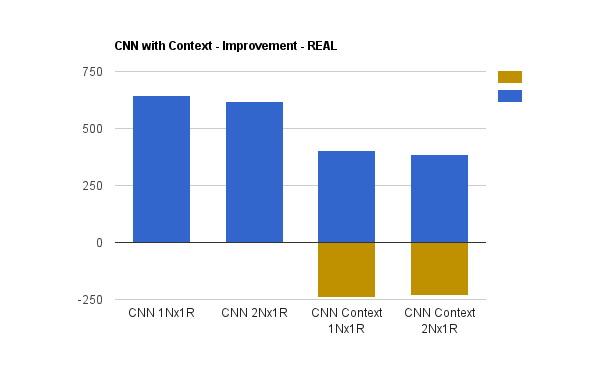
\includegraphics[width=\columnwidth]{imgs/cxtCNN-R.png}
	\caption{Improvements on Simulated dataset for CNN-SLOC when temporal context is considered.}
	\label{fig:cxtCNN-S}
\end{figure}

%The introduction of the temporal context has beneficial effects also with the MLP, but with a lower error reduction (equal to 21.5\%).

In this case the CNN results more effective with respect to the MLP architecture, and it is able to further reduce the RMSE,
%ndFAB Results discussion - 6c)
\textcolor{red}{{as we can notice from the table \tableref{tab:bestCONF_SIMU}.}}
In particular, the CNN-2Rx1N architecture reduces the RMSE by 37\% with respect to the method proposed in a previous work by the authors \cite{vesperini2016sloc}.
Indeed, the introduction of a temporal context improves the performance also with the MLP architecture, with an RMSE reduction equal to 21.5\%.

The  results obtained in the investigation of the audio excerpt are reported in \figref{ctx-str-SIMU}, where the values of the RMSE for different strides $s$ are plotted while varying the temporal context $C$. %It can be noticed that a similar trend of performance with respect to temporal resolution values is registered.
%ndFAB Results discussion - 6c)
%It can be noticed that a similar trend of performance with respect to temporal resolution \textcolor{red}{{(i.e., equal to $C\cdot s$)}} of the input values is registered.
%%
\textcolor{red}{Observing the results related to the MLP-SLOC (\figref{sfig:mlp-real-context}), it can be noticed that increasing the context size $C$ up to 15 (stride equal to 3), 17 (stride equal to 5), or 19 (stride 1 and 4) reduces the RMSE. Regarding the behavior for different values of the stride, a part from the results related to stride equal to 1, the performance difference is negligible, since it amounts at most to 1.93\,mm. Similar considerations apply to the behavior of CNN-SLOC for different sizes of the temporal context and of the stride (\figref{sfig:cnn-real-context}).}

\begin{figure}[t] 
	\centering
	\begin{subfigure}{0.45\columnwidth}	
	\pgfplotsset{
		%legend style={legend pos=north east}
		legend style={
			at={(1.15,1.05)},
			anchor=north east,
		},
	}%
	\centering
	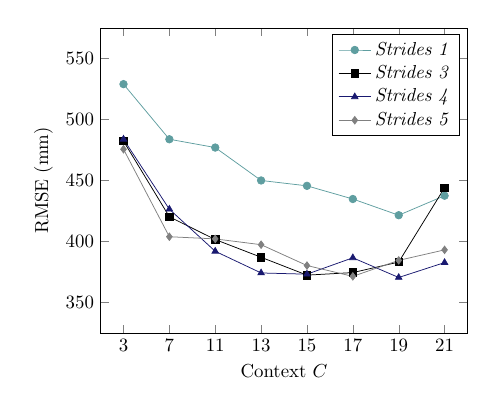
\begin{tikzpicture}[scale=0.68]
	\begin{axis}[
	xmax=7.5,xmin=-0.5,
	ymin= 325,ymax=575,
	title=,ylabel=RMSE (mm),xlabel={Context $C$},
	xtick={0,1,...,7},
	xticklabels={3,7,11,13,15,17,19,21},
	ytick={350,400,...,550},
	]
	%marks = * triangle square x pentagon diamond
	
	\addplot [draw = CadetBlue, mark = *, CadetBlue] coordinates{(0,529) (1,483.8) (2,477) (3,450) (4,445.6) (5,434.8) (6,421.5) (7,437.5)};
	\addplot [draw = Black, mark = square*, Black] coordinates{(0,482.29) (1,420.22) (2,401.57) (3,387.03) (4,372.37) (5,374.46) (6,383.1) (7,444.07)};
	\addplot [draw = MidnightBlue, mark =triangle*, MidnightBlue] coordinates{(0,483.81) (1,426.44) (2,391.93) (3,374.15) (4,373.16) (5,386.6) (6,370.44) (7,382.67)};
	\addplot [draw = Gray, mark =diamond*, Gray] coordinates{(0,475.64) (1,403.87) (2,402.08) (3,397.34) (4,380.25) (5,371.35) (6,384.48) (7,393.09)};
	
	\legend{\emph{Strides 1},\emph{Strides 3},\emph{Strides 4},\emph{Strides 5}}
	\end{axis}
	\end{tikzpicture}%
		\caption{Results related to MLP-SLOC algorithm.}\label{sfig:mlp-real-context}
	\end{subfigure}
	%
	%
	\hfill
	\begin{subfigure}{0.45\columnwidth}	
		\pgfplotsset{
			%legend style={legend pos=north east}
			legend style={
				at={(1.15,1.05)},
				anchor=north east,
			},
		}%
			\centering
	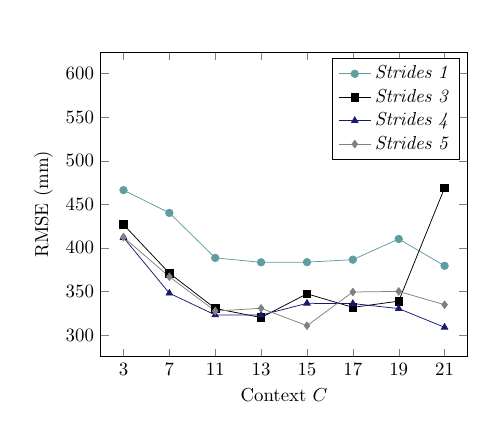
\begin{tikzpicture}[scale=0.68]
	\begin{axis}[
	xmax=7.5,xmin=-0.5,
	ymin= 275,ymax=625,
	title=\emph{},ylabel=RMSE (mm),xlabel={Context $C$},
	xtick={0,1,...,7},
	xticklabels={3,7,11,13,15,17,19,21},
	ytick={300,350,...,600},
	]
	%marks = * triangle square x pentagon diamond
	
	\addplot [draw = CadetBlue, mark = *, CadetBlue] coordinates{(0,466.28) (1,440.11) (2,388.49) (3,383.4) (4,383.6) (5,386.43) (6,410.2) (7,379.4)};
	\addplot [draw = Black, mark = square*, Black] coordinates{(0,426.7) (1,370.89) (2,330.41) (3,320) (4,347.24) (5,331.67) (6,338.79) (7,468.84)};
	\addplot [draw = MidnightBlue, mark =triangle*, MidnightBlue] coordinates{(0,411.87) (1,347.91) (2,322.94) (3,322.76) (4,336.3) (5,336.04) (6,330.29) (7,308.79)};
	\addplot [draw = Gray, mark =diamond*, Gray] coordinates{(0,412.31) (1,366.82) (2,327.48) (3,330.62) (4,310.63) (5,349.32) (6,350) (7,334.71)};
	\legend{\emph{Strides 1},\emph{Strides 3},\emph{Strides 4},\emph{Strides 5}}
	\end{axis}
	\end{tikzpicture}%
	\caption{Results related to CNN-SLOC algorithm.}
		\end{subfigure}
	%
	%
	%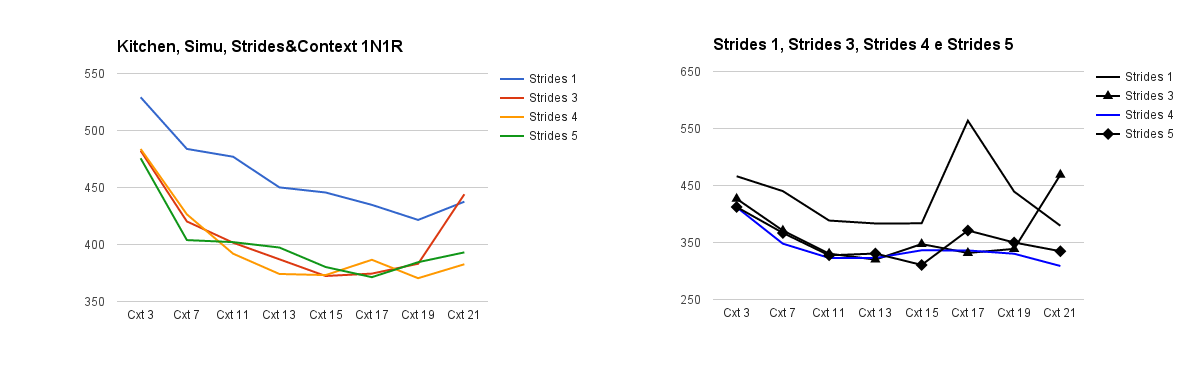
\includegraphics[width=0.8\textwidth]{imgs/cxtSIMU.png}
	\caption{Performance trend in the Simulated dataset for different values of the stride $s$ and context size $C$. The results are related to the Kitchen room and they have been obtained by using the 1Rx1N architecture.}\label{sfig:cnn-real-context}
	\label{ctx-str-SIMU}
\end{figure}




\subsection{Results on the Real Dataset} 
The main difference between the Real and the Simulated  dataset is the position of the speaker, which is not fixed during the scene. Thus, the speaker moves within the room while pronouncing the sentence. Furthermore, in this dataset overlapping events are not present.
\begin{table}[!h]
	\centering
	\caption{Comparison of best results of SLOC algorithms in terms of RMSE (mm) and $P_{cor}$ (\%) in the Real case study. The temporal context is espressed in terms of $C$ - $s$ (frames), respectively the total length of the chunk and the stride.}
	\label{tab:results_REAL}
	%\renewcommand{\arraystretch}{1.1}
	\resizebox{\columnwidth}{!}{
		\begin{tabular}{l|ccc|ccc|cc}
			\hline
			\hline
			\multicolumn{9}{c}{REAL}                                                                                                                                                                                                                               \\
			\hline
			ROOM      & \multicolumn{3}{c|}{Kitchen}                                                            & \multicolumn{3}{|c|}{Living Room}                                                        & \multicolumn{2}{c}{Average}                              \\
			\hline
			& \multicolumn{1}{l}{ $C$ - $s$ (frames)} & \multicolumn{1}{r}{RMSE (mm)} & \multicolumn{1}{l|}{$P_{cor}$ (\%)} & \multicolumn{1}{l}{ $C$ - $s$ (frames)} & \multicolumn{1}{l}{RMSE (mm)} & \multicolumn{1}{l|}{$P_{cor}$ (\%)} & \multicolumn{1}{l}{RMSE (mm)} & \multicolumn{1}{l}{$P_{cor}$ (\%)} \\
			\hline
			\hline
			MLP 1Rx1N & /                          & 789                      & 39                            & /                          & 688                      & 43                            & 644                      & 42                            \\
			MLP 1Rx1N & 19 - 3                      & 498                      & 60                            & 21 - 4                      & 446                      & 63                            & 472                      & 61                            \\ \hline
			MLP 2Rx1N & /                          & 710                      & 38                            & /                          & 619                      & 45                            & 664                      & 41                            \\
			MLP 2Rx1N & 21 - 4                      & 494                      & 59                            & 17 - 4                      & 445                      & 63                            & 470                      & 61                            \\ \hline
			CNN 1Rx1N & /                          & 706                      & 37                            & /                          & 583                      & 47                            & 686                      & 42                            \\
			CNN 1Rx1N & 21 - 3                      & 460                      & 64                            & 15 - 5                      & 349                      & 78                            & 620                      & 71                            \\ \hline
			CNN 2Rx1N & /                          & 687                      & 40                            & /                          & 552                      & 54                            & 470                      & 61                            \\
			CNN 2Rx1N & 19 - 4                      & 425                      & 72                            & 17 - 3                      & 350                      & 75                            & 387                      & 74                            \\ \hline
			CSP-SLOC  & /                          & 1394                     & 9                             & /                          & 1166                     & 11                            & 1280                     & 10                            \\ \hline
			SRP-SLOC  & /                          & 895                      & 30                            & /                          & 690                      & 53                            & 793                      & 42                                                  
			
		\end{tabular}
	}
\end{table}


\subsubsection{Evaluation without the temporal context}
\tableref{tab:results_REAL} reports a comparison among the evaluated algorithms with the best results obtained for each configuration. As in \tableref{tab:results_SIMU}, for the DNN-SLOC, both the performance are reported without temporal context and at the end of the fourth stage, in which performance have been studied investigating the temporal context.

The localization performance obtained by the CSP-SLOC algorithm is quite similar to the one in the Simulated case study, with an average RMSE equal to 1280\,mm. The SRP-PHAT algorithm attains an averaged RMSE equal to 792\,mm. The performance achieved by the comparative methods is significantly superior than the one obtained in the Simulated case study. The motivation is the higher SNR level characterizing the audio files in the Real dataset.

\begin{figure}[t]
	\centering
	\begin{tikzpicture}[scale=0.8]
	
	\begin{axis}[
	%legend entries = {1Rx1N, 2Rx1N},
	% legend to name={legend},
	title = Real Dataset - GCC SELECTION,
	boxplot/draw direction=y,
	x axis line style={opacity=0},
	axis x line*=bottom,
	axis y line=left,
	enlarge y limits,
	ymajorgrids,
	%xtick={1,3,5,7},
	%xticklabel style = {font=\tiny},
	xtick={1.5,3.5},
	xticklabels={CNN, MLP},
	ylabel={RMSE (\%)},
	ytick={},ymin=618,ymax=810]
	]
	%BLUE MLP
	%RED CNN
	\addplot+[
	boxplot prepared={
		median=677,
		upper quartile=684,
		lower quartile=670,
		upper whisker=710,
		lower whisker=654
	},fill=BoxCol,draw=BoxCol,fill opacity=0.8, 
	] coordinates {};
	%\addlegendentry{1Rx1N}
	\addplot+[
	boxplot prepared={
		median=643,
		upper quartile=638,
		lower quartile=648,
		upper whisker=662,
		lower whisker=619
	}, fill=BoxCol1,draw=BoxCol1,fill opacity=0.8,
	] coordinates {};
	%\addlegendentry{2Rx1N}
	\addplot+[
	boxplot prepared={
		median=773,
		upper quartile=782,
		lower quartile=764,
		upper whisker=807,
		lower whisker=739
	}, fill=BoxCol,draw=BoxCol,fill opacity=0.8
	] coordinates {};
	\addplot+[
	boxplot prepared={
		median=687,
		upper quartile=694,
		lower quartile=680,
		upper whisker=714,
		lower whisker=661
	}, fill=BoxCol1,draw=BoxCol1,fill opacity=0.8
	] coordinates {};
	% \node [above left]  at (rel axis cs:0.9,0.2) {\ref{legend}};
	\end{axis}
	
	\begin{customlegend}[legend entries={1Rx1N, 2Rx1N}, legend style={at={(2.5,5.4)}} ]
	\addlegendimage{BoxCol,fill=BoxCol,fill opacity=0.8,area legend}
	\addlegendimage{BoxCol1,fill=BoxCol1,fill opacity=0.8,area legend}
	\end{customlegend}
	
	\end{tikzpicture}
	
	\caption{Boxplot for the Real dataset, for MLP and CNN neural network, comparing 1Rx1N and 2Rx1N setups. This evaluation is performed at the end of the second stage of optimization, considering all the tested GCC Patterns configurations. The results are averaged over the two target rooms.}
	\label{fig:boxplot_real-mlp}
\end{figure}
As shown in \figref{fig:boxplot_real-mlp}, in this case the 2Rx1N architecture produces a more significant improvement of performance both for the MLP-SLOC and the CNN-SLOC, and consistently with what observed for the Simulated dataset, the variance with the microphone position decreases.
As result of the third optimization stage, the best performing MLP layout in the 2Rx1N case is composed of a single layer of 16 units  both for the Kitchen and the Living Room. Regarding the CNN-SLOC,  the most performing configuration is composed of a convolutional layer with 24 $5\times5$ kernels without pooling, followed by a two layers MLP with respectively 256, 256 units and 256, 512 units for Kitchen and Living Room.

\begin{table}[t]
	\centering
	\caption{Results for Convolutional Neural Networks with the best performing configurations in the Real case study.}
	\label{tab:bestCONF_REAL}
		\resizebox{\columnwidth}{!}{
	\begin{tabular}{c|cc|cl|cc|cc|cc}
		%\cline{2-11}
		\multicolumn{1}{l|}{}                       & \multicolumn{2}{c|}{Features Settings}                    & \multicolumn{2}{c|}{Microphones}                                                                                            & \multicolumn{2}{c|}{\begin{tabular}[c]{@{}c@{}}Convolutional \\ Kernels\end{tabular}} & \multicolumn{2}{c|}{Feed Forward Layers}    & \multicolumn{2}{c}{Results}               \\ \hline
		\multicolumn{1}{c|}{\multirow{2}{*}{Room}} & \multirow{2}{*}{Configuration} & \multirow{2}{*}{ $C$ - $s$ (frame)} & \multicolumn{1}{c}{\multirow{2}{*}{Ceiling}}                                  & \multicolumn{1}{c|}{\multirow{2}{*}{Wall}} & \multirow{2}{*}{Number}                 & \multirow{2}{*}{Size}                       & First                & Second               & RMSE                 & $P_{cor}$           \\
		
		\multicolumn{1}{c|}{}                      &                                &                          & \multicolumn{1}{c}{}                                                          & \multicolumn{1}{c|}{}                      &                                         &                                             & Layer                & Layer                & (mm)                 & (\%)                \\ \hline
		\hline
		\multirow{6}{*}{Kitchen}                    & \multirow{6}{*}{2Rx1N}         & \multirow{6}{*}{19 - 4}  & \multirow{3}{*}{\begin{tabular}[c]{@{}c@{}}Circular \\ Array (K)\end{tabular}}  & \multicolumn{1}{c|}{K1R,K1L}               & \multirow{6}{*}{24}                     & \multirow{6}{*}{$5\times5$}                 & \multirow{6}{*}{256} & \multirow{6}{*}{256} & \multirow{6}{*}{425} & \multirow{6}{*}{72} \\
		&                                &                          &                                                                            & K3L,K3C                                    &                                         &                                             &                      &                      &                      &                     \\
		&                                &                          &                                                                            & K3L,K3C                                    &                                         &                                             &                      &                      &                      &                     \\
		&                                &                          & \multirow{3}{*}{\begin{tabular}[c]{@{}c@{}}Circular \\ Array (L)\end{tabular}} & L1C,L1L                                    &                                         &                                             &                      &                      &                      &                     \\
		&                                &                          &                                                                            & L2L,L2R                                    &                                         &                                             &                      &                      &                      &                     \\
		&                                &                          &                                                                                & L3L,L3R                                    &                                         &                                             &                      &                      &                      &                     \\ \hline
		\multirow{4}{*}{Living Room}                & \multirow{4}{*}{2Rx1N}         & \multirow{4}{*}{17 - 3}  & \multirow{2}{*}{\begin{tabular}[c]{@{}c@{}}Circular\\ Array (K)\end{tabular}}  & \multicolumn{1}{c|}{K2L,K2R}               & \multirow{4}{*}{24}                     & \multirow{4}{*}{$5\times5$}                 & \multirow{4}{*}{256} & \multirow{4}{*}{512} & \multirow{4}{*}{350} & \multirow{4}{*}{75} \\
		&                                &                          &                                                                                & K3C,K3R                                    &                                         &                                             &                      &                      &                      &                     \\
		&                                &                          & \multirow{2}{*}{\begin{tabular}[c]{@{}c@{}}Circular \\ Array (L)\end{tabular}} & L2L,L2R                                    &                                         &                                             &                      &                      &                      &                     \\
		&                                &                          &                                                                                & L1R,L1C                                    &                                         &                                             &                      &                      &                      &                    
	\end{tabular}
	}
\end{table}

\subsubsection{Evaluation including the temporal context}

As performed with the Simulated dataset, the effects of the temporal context have been studied after the third optimization stage.  The introduction of the temporal context leads to an average localization accuracy of 387\,mm with the CNN-SLOC for the 2Rx1N configuration. As highlighted in \figref{fig:cxtCNN-R}, the RMSE reduces by 37.2\% for the 1Rx1N configuration and by 37.5\% for the 2Rx1N configuration. In concordance with the results obtained with the Simulated dataset, the MLP architecture benefits from the introduction of the temporal context, with a resulting error reduction of 36\% for the 1Rx1N and of 29\% for the 2Rx1N configuration.


For the CNN-SLOC applied in the Real dataset, the best resulting values of context and strides are $(C,s)=(19,4)$ and $(C,s)=(17,3)$ respectively for Kitchen and Living Room, corresponding to segments of length \textcolor{red}{0.75\,s and 0.51\,s.} 


\figref{ctx-str-REAL} reports the RMSE for different context sizes $C$ and strides $s$ in the case of 1Rx1N applied to the Kitchen room.
%It is noticeable the similar trend of the performance while varying the temporal resolution. 
Similarly to the \textit{Simulated} dataset, the variation of the temporal resolution produces a similar performance trend for the two neural architectures. 
Details of the best performing configurations are provided in \tableref{tab:bestCONF_REAL}.


\begin{figure}[!h]
	\centering
	\begin{tikzpicture}[scale=0.8]
	
	\begin{axis}[
	ybar,
	bar width=23pt,
	x axis line style={opacity=0},
	%grid = both
	axis x line*=bottom,
	axis y line=left,
	title style={at={(0.28,1.00)}},
	title = {Real Dataset - CNN-SLOC},
	enlarge y limits,
	ymajorgrids,
	xticklabel style={align=center}, xticklabel style = {font=\footnotesize},
	xtick={1.25,2.55,5.25,6.55},xmin=0.5,xmax=7.5,
	xticklabels={Without \\ Context, With\\Context, Without \\ Context, With\\Context},
	ylabel={RMSE (mm)},
	ytick={0,150,...,600},ymin=0,ymax=675
	]
	
	\addplot [ draw = BoxCol, fill = BoxCol, fill opacity=1] 	coordinates {(2-0.3,644)  (3,405) };
	\addplot [ draw = BoxCol1, fill = BoxCol1, fill opacity=1] 	coordinates {(5-0.25,620)  (6+0.1,387)};
	
	\draw (axis cs:3.25-0.7,405) -- node[right]{42\%} (axis cs:3.25-0.7,644);
	\draw (axis cs:3-0.7,405) -- (axis cs:3.5-0.7,405);
	\draw (axis cs:3-0.7,644) -- (axis cs:3.5-0.7,644);
	
	\draw (axis cs:7.25-0.7,387) -- node[right]{39\%} (axis cs:7.25-0.7,620);
	\draw (axis cs:7.0-0.7,387) -- (axis cs:7.5-0.7,387);
	\draw (axis cs:7.0-0.7,620) -- (axis cs:7.5-0.7,620);	
	
	\end{axis}
	
	\begin{customlegend}[legend entries={1Rx1N, 2Rx1N, Improvement}, legend style={at={(6.8,6.6)}} ]
	\addlegendimage{BoxCol,fill=BoxCol,fill opacity=1,area legend}
	\addlegendimage{BoxCol1,fill=BoxCol1,fill opacity=1,area legend}
	\end{customlegend}
	\end{tikzpicture}
	
	\caption{Improvements on Real dataset for CNN-SLOC when temporal context is considered.}
	\label{fig:cxtCNN-R}
\end{figure}

\begin{figure}[!h]
	\centering
	\pgfplotsset{
		%legend style={legend pos=north east}
		legend style={
			at={(1.15,1.05)},
			anchor=north east,
		},
	}%
	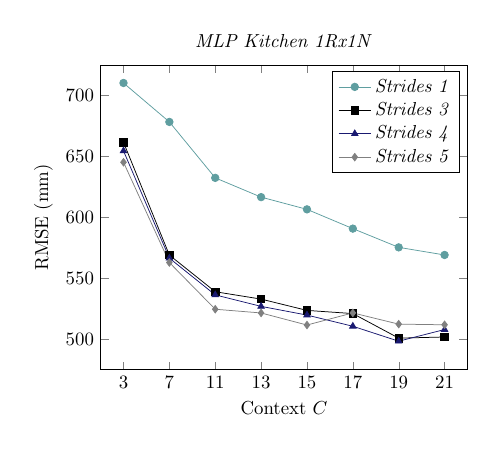
\begin{tikzpicture}[scale=0.68]
	\begin{axis}[
	xmax=7.5,xmin=-0.5,
	ymin= 475,ymax=725,
	title=\emph{MLP Kitchen 1Rx1N},ylabel=RMSE (mm),xlabel={Context $C$},
	xtick={0,1,...,7},
	xticklabels={3,7,11,13,15,17,19,21},
	ytick={500,550,...,700},
	]
	%marks = * triangle square x pentagon diamond			
	\addplot [draw = CadetBlue, mark = *, CadetBlue] coordinates{(0,710.21) (1,678.28) (2,632.41) (3,616.6) (4,606.58) (5,590.78) (6,575.42) (7,569.17)};
	\addplot [draw = Black, mark = square*, Black] coordinates{(0,661.59) (1,569.08) (2,539.02) (3,532.98) (4,523.71) (5,521.12) (6,500.98) (7,501.91)};							
	\addplot [draw = MidnightBlue, mark =triangle*, MidnightBlue] coordinates{(0,654.52) (1,566.56) (2,536.41) (3,527.02) (4,519.88) (5,510.71) (6,498.45) (7,508.03)};							
	\addplot [draw = Gray, mark =diamond*, Gray] coordinates{(0,645.22) (1,562.98) (2,524.67) (3,521.61) (4,511.72) (5,521.65) (6,512.45) (7,511.92)};   							
	\legend{\emph{Strides 1},\emph{Strides 3},\emph{Strides 4},\emph{Strides 5}}
	\end{axis}
	\end{tikzpicture}%
	~%
	%
	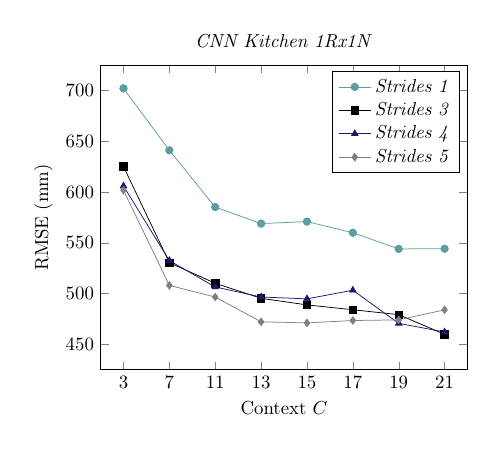
\begin{tikzpicture}[scale=0.68]
	\begin{axis}[
	xmax=7.5,xmin=-0.5,
	ymin= 425,ymax=725,
	title=\emph{CNN Kitchen 1Rx1N},ylabel=RMSE (mm),xlabel={Context $C$},
	xtick={0,1,...,7},
	xticklabels={3,7,11,13,15,17,19,21},
	ytick={450,500,...,700},
	]
	\addplot [draw = CadetBlue, mark = *, CadetBlue] coordinates{(0,701.97) (1,640.97) (2,585.13) (3,568.89) (4,570.86) (5,559.88) (6,543.96) (7,544.14)};
	\addplot [draw = Black, mark = square*, Black] coordinates{(0,625.01) (1,530.43) (2,510.14) (3,495.35) (4,488.86) (5,484.09) (6,479.26) (7,459.93)};
	\addplot [draw = MidnightBlue, mark =triangle*, MidnightBlue] coordinates{(0,605.82) (1,532.48) (2,506.5) (3,496.63) (4,494.81) (5,503.31) (6,470.7) (7,462.18)};
	\addplot [draw = Gray, mark =diamond*, Gray] coordinates{(0,601.69) (1,508.08) (2,496.59) (3,472.23) (4,471.15) (5,473.51) (6,474.12) (7,484.02)};
	\legend{\emph{Strides 1},\emph{Strides 3},\emph{Strides 4},\emph{Strides 5}}
	\end{axis}
	\end{tikzpicture}%
	~%
	%
	\caption{Performance trend in the Real dataset for different \textit{strides} at growing \textit{context}. The considered room is Kitchen with 1Rx1N configuration, the two DNN are plotted.}
	\label{ctx-str-REAL}
\end{figure}

\subsection{Computational complexity}
The computational complexity of the proposed approach and of the comparative methods has been calculated taking as reference the computational complexity 

\section{Conclusion and Outlook}
\label{sec:concl}

In this paper, a DNN-based approach for speaker localization in a multi-room domestic environment has been proposed and an extensive evaluation of the performance has been performed. The neural network employs GCC-PHAT Patterns as input features, obtained by combining the signals acquired with several microphone pairs. Hence, two different neural network architectures have been investigated, the multi layer perceptron (MLP) and the convolutional neural network (CNN). The coordinates of a speaker inside the target room are directly estimated without additional processing, resulting in a fully data-driven approach.
A particular effort has been directed to the evaluation of a spatial and temporal context, revealing the latter to be extremely decisive. \textcolor{red}{In details, the capability of the network to exploit the audio coming from all the rooms has been evaluated, and different numbers of adjacent frames have been concatenated to evaluate the influence of the temporal context.}
%%
\textcolor{red}{The algorithm implicitly requires an Oracle multi-room VAD that identifies the time boundaries of the audio signals and the source room.} The performance have been evaluated on the DIRHA Dataset and compared to two state-of-the-art algorithm, based respectively on Crosspower Spectrum Phase estimation (CSP-SLOC) and on Steered Response Power (SRP-SLOC).

In terms of absolute improvement, compared to the SRP-SLOC approach, the CNN-SLOC improves the performance by 66\% and 51\% respectively for the Simulated and the Real dataset. With regards to the two evaluated neural network architectures, the CNN with 3-D kernels is able to exploit the temporal context information more efficiently respect to the MLP network both in terms of RMSE and $P_{cor}$.
%The proposed method operates in a complete autonomous way. Indeed, once trained, the neural network provides the coordinates of the speaker directly from the speech excerpts of the signals captured by the microphone arrays. This allows to totally avoid the fine-tuning of parameters being generally needed by state-of-the-art approaches, which depends on the application environment and implicates a lack of generality.
\textcolor{red}{An advantage of the proposed approach with respect to the CSP-SLOC and SRP-SLOC algorithms is its less dependence on the characteristics of the environment: indeed, CSP-SLOC and SRP-SLOC require respectively the knowledge of the microphones position and the knowledge of the room geometry, while the proposed approach infers this information directly from the data. Regarding the hyperparameters, all the algorithms require their manual or automatic tuning in order to obtain the lowest localization error. In particular, the proposed approach requires choosing the hyperparameters of the network, the size of the context and the stride, and a microphone selection stage. The hyperparameters of the network mostly dependent on the size of the training set. However, it is worth highlighting the microphone selection stage and the context evaluation stage are important for obtaining the best overall performance, but they are not fundamental for obtaining a significant performance improvement with respect to the comparative methods. In particular, the highest RMSE of CNN-SLOC with the 2Rx1N architecture and without using the temporal context and microphone selection is lower than the SRP-SLOC RMSE in both datasets: 286\,mm in the simulated dataset (see \figref{fig:boxplot_simu-mlp} and \tableref{tab:results_SIMU}) and 131\,mm in the real dataset (\figref{fig:boxplot_real-mlp} and \tableref{tab:results_REAL}).}

%\textcolor{red}{{Differently, a lack of generality is observed in the proposed state-of-the-art approaches. For example, the CSP-SLOC requires the knowledge of the room geometry, in addition, parameters such as iterations and number of searched maxima has been fine-tuned for the SRP-SLOC.}}

\textcolor{red}{
Due to the lack of a suitable dataset, it was not possible to evaluate the performance of the proposed approach in environments that differ from the one used during the training phase. Future works will address this aspect by creating a new multi-room dataset, as well as the possibility of using transfer learning methods to adapt the trained models to new environments \cite{Pan2010}. Additionally, future works will be oriented to the development of a joint multi-room VAD \cite{ijcnn-vad,ijcnn2016-vad} and SLOC neural network based system, in order to obtain an integrated and fully data-driven algorithm. Finally, different neural networks will be investigated, with a deeper focus on the temporal evolution of the signal by means of a temporal context, such as Long Short Term Memory (LSTM) Neural Networks \cite{hochreiter1997long}.}

\section*{Acknowledgement}
This research has been partly supported by the Italian University and Research Consortium CINECA. We acknowledge the CINECA award under the ISCRA initiative, for the availability of high performance computing resources and support.



%% The Appendices part is started with the command \appendix;
%% appendix sections are then done as normal sections
%% \appendix

%% \section{}
%% \label{}

%% References
%%
%% Following citation commands can be used in the body text:
%% Usage of \cite is as follows:
%%   \cite{key}         ==>>  [#]
%%   \cite[chap. 2]{key} ==>> [#, chap. 2]
%%

%% References with BibTeX database:

\bibliographystyle{elsarticle-num}
\bibliography{mybib}

%% Authors are advised to use a BibTeX database file for their reference list.
%% The provided style file elsarticle-num.bst formats references in the required Procedia style

%% For references without a BibTeX database:

% \begin{thebibliography}{00}

%% \bibitem must have the following form:
%%   \bibitem{key}...
%%

% \bibitem{}

% \end{thebibliography}
\newpage
\section*{Author biographies}


\parpic{{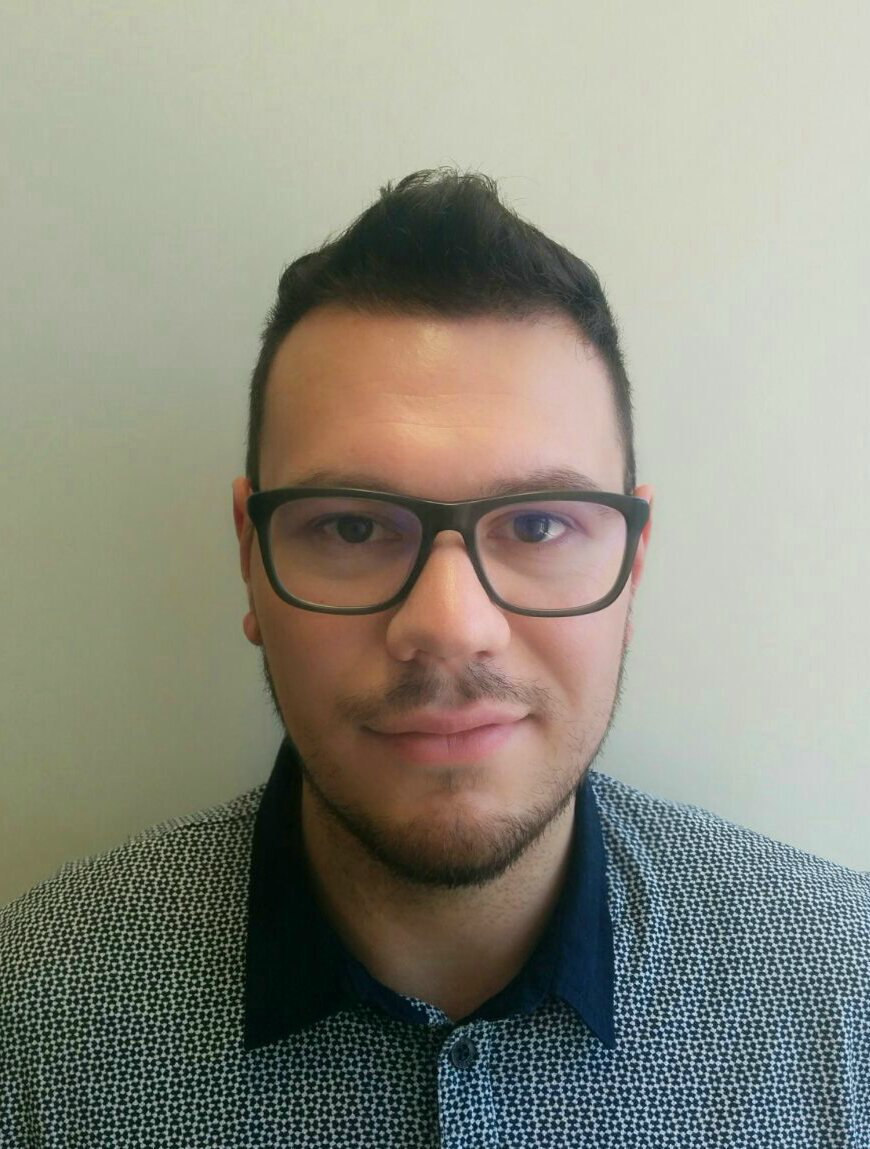
\includegraphics[width=1in,height=1.25in,clip,keepaspectratio]{pictures/fabio_vesperini.jpg}}}
\noindent {\bf Fabio Vesperini} was born in San Benedetto del Tronto, Italy, on May 1989. He received his M.Sc. degree (cum laude) in electronic engineering in 2015 from Universit\`{a} Politecnica delle Marche (UnivPM). In 2014 he was at the Technische Universtit\"at M\"unchen as visiting student for 7 months, where he carried out his master thesis project on acoustic novelty detection. He is currently a PhD student at the Department of Information Engineering, at UnivPM. His research interests are in the fields of digital signal processing and machine learning for intelligent audio analysis.
\vspace{1cm}

\parpic{{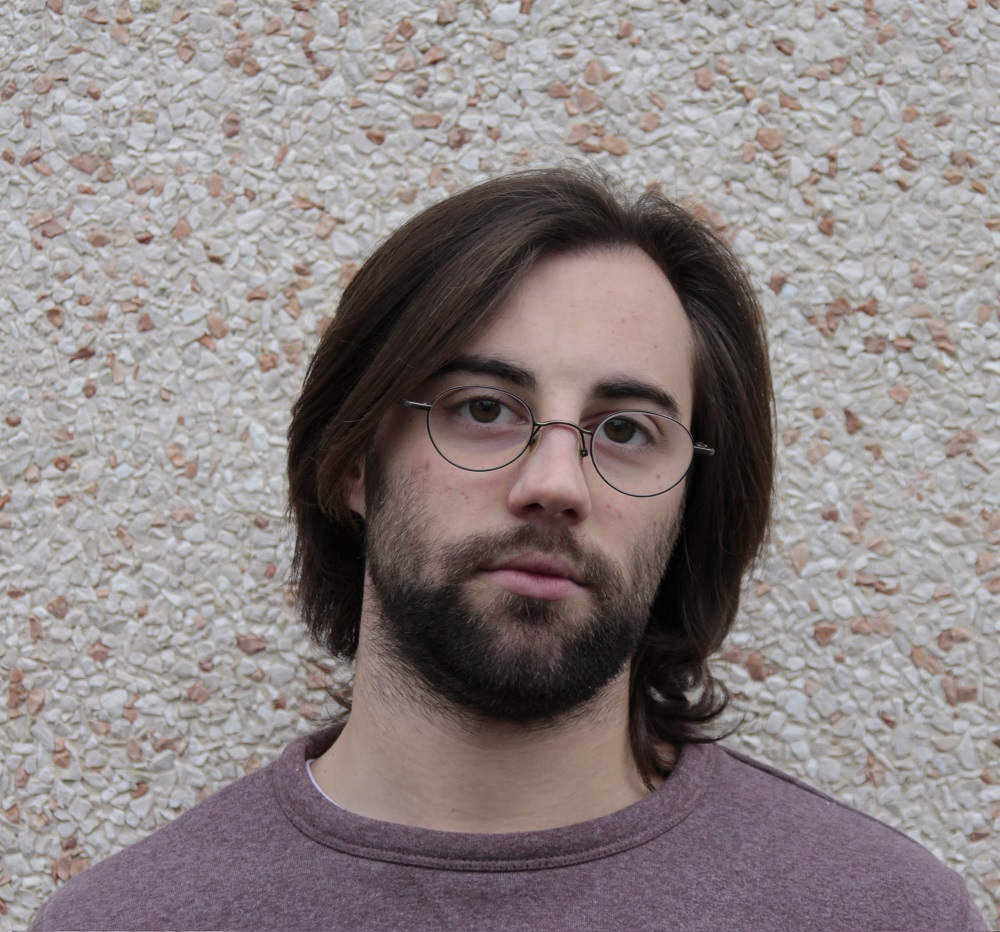
\includegraphics[width=1in,height=1.25in,clip,keepaspectratio]{pictures/paolo.jpg}}}
\noindent {\bf Paolo Vecchiotti} was born in Senigallia, Italy, on October 1991. He received his M.Sc. degree (cum laude) in Electronic Engineering in 2015 at Universit\`{a} Politecnica delle Marche (UnivPM). In 2013 he spent 5 months at the Fachhochschule K\"arnten for an Erasmus project. He is currently a PhD student at the Department of Information Engineering, at UnivPM. His research in focused on Computational Audio Processing.
\vspace{1cm}

\parpic{{
\includegraphics[width=1in,height=1.25in,clip,keepaspectratio]{pictures/emap_pic.png}}}
\noindent {\bf Emanuele Principi} was born in Senigallia (Ancona), Italy, on January 1978. He received the M.S. degree in electronic engineering (with honors) from Universit\`a Politecnica delle Marche (Italy) in 2004. He received his Ph.D. degree in 2009 in the same university under the supervision of Prof. Francesco Piazza. In November 2006 he joined the 3MediaLabs research group coordinated by Prof. Francesco Piazza at Universit\`a Politecnica delle Marche where he collaborated to several regional and european projects on audio signal processing. Dr. Principi is author and coauthor of several international scientific peer-reviewed articles in the area of speech enhancement for robust speech and speaker recognition and intelligent audio analysis. He is member of the IEEE CIS Task Force on Computational Audio Processing, and is reviewer for several international journals. His current research interests are in the area of machine learning and digital signal processing for the smart grid (energy task scheduling, non-intrusive load monitoring, computational Intelligence for vehicle to grid) and intelligent audio analysis (multi-room voice activity detection and speaker localization, acoustic event detection, fall detection).
\vspace{1cm}

\parpic{{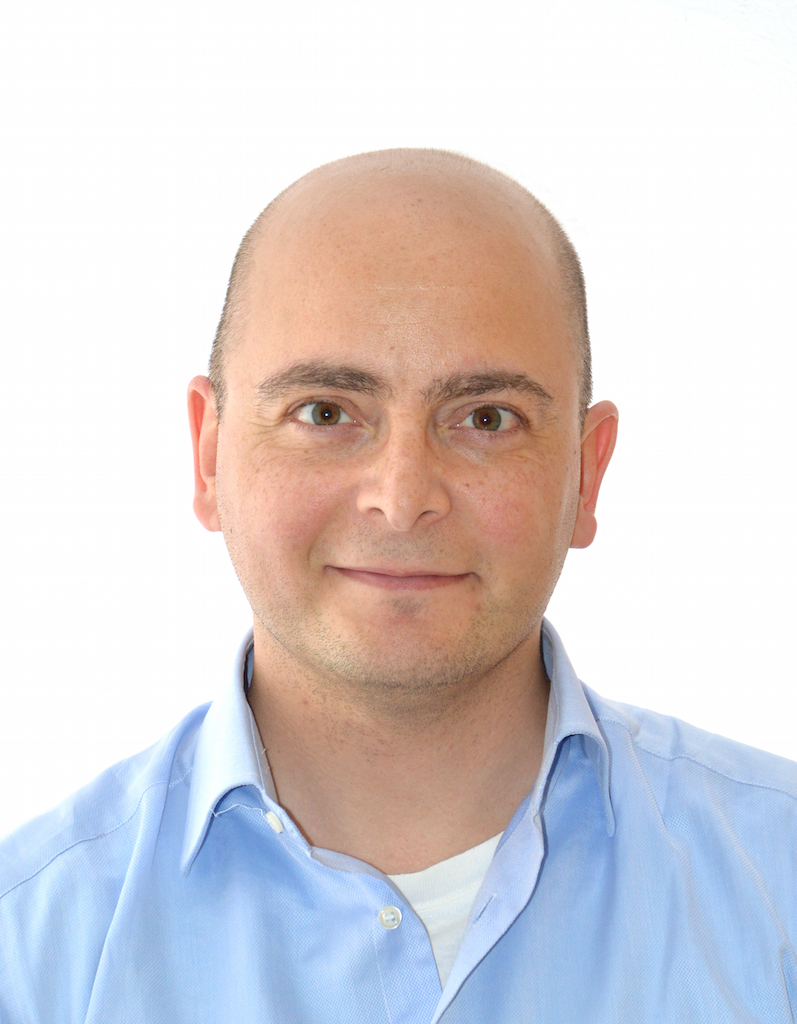
\includegraphics[width=1in,height=1.25in,clip,keepaspectratio]{pictures/Stefano_Squartini.jpg}}}
\noindent {\bf Stefano Squartini} was born in Ancona, Italy, on March 1976. He got the Italian Laurea with honors in electronic engineering from University of Ancona (now Universit\`{a} Politecnica delle Marche, UnivPM), Italy, in 2002. He obtained his PhD at the same university in 2005. He joined the Department of Information Engineering at UnivPM as Assistant Professor (2007), and then as Associate Professor in Circuit Theory (2014). His current research interests are in the area of digital signal processing and computational intelligence, with focus on speech/audio processing and energy management. He is author and coauthor of more than 160 international scientific peer-reviewed articles. He was Associate Editor for the IEEE Transactions on Neural Networks and Learning Systems (2010-2016) and is currently member of the Cognitive Computation, Big Data Analytics and Artificial Intelligence Reviews Editorial Boards (starting from 2011, 2014 and 2016, respectively). He is the Organizing Chair of the IEEE CIS Task Force on Computational Audio Processing.
\vspace{1cm}

\parpic{{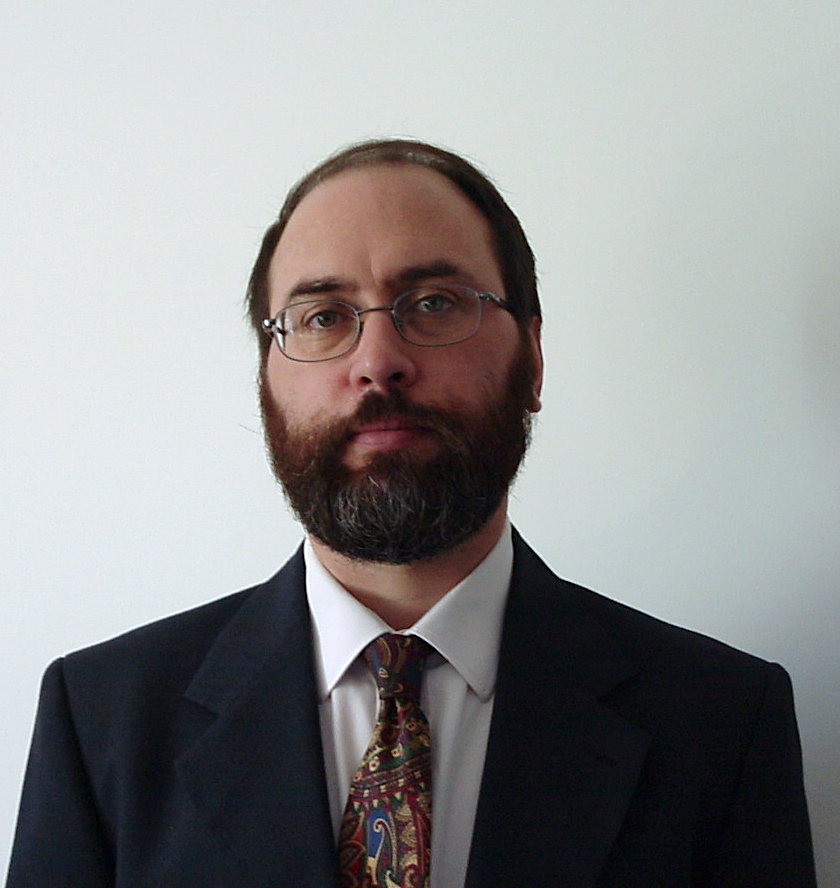
\includegraphics[width=1in,height=1.25in,clip,keepaspectratio]{pictures/Francesco_Piazza.jpg}}}
\noindent {\bf Francesco Piazza} was born in Jesi, Italy, on February 1957. He got the Italian Laurea with honors in electronic engineering from the University of Ancona, Italy, in 1981. From 1981 to 1983 he worked on image processing at the Physics Department. In 1983 he worked at the Olivetti OSAI software development center (Ivrea, Italy). In 1985 he joined the Department of Electronics and Automatics of the University of Ancona. Currently he is Full Professor of Electrical Science and Director of the Department of Information engineering at the Universit\`{a}  Politecnica delle Marche, in Italy.
He is author or coauthor of more than 350 international papers. His current research interests are in the areas of circuit theory and digital signal processing including adaptive DSP algorithms and circuits, artificial neural networks, speech and audio processing. 


\end{document}

%%
%% End of file `ecrc-template.tex'. 